%% ==========================================================================
%%  Patient-aware agentic cyber-resilience for the Internet of Medical Things
%%  Elsevier single-column (elsarticle, preprint, 12pt).  Self-contained:
%%  figures are TikZ/pgfplots with the measured data embedded, and the
%%  bibliography is inline, so it compiles as one file (Overleaf: pdfLaTeX).
%%
%%  Search for "TODO" before submitting: corresponding author / e-mail, the
%%  target journal's own template (change only the \documentclass line and the
%%  frontmatter block), and the "VERIFY" notes on the related-work table.
%% ==========================================================================
\documentclass[preprint,12pt]{elsarticle}

\usepackage[utf8]{inputenc}
\usepackage{amsmath,amssymb}
\usepackage{booktabs,array,multirow,tabularx,longtable,needspace}
\usepackage{graphicx}
\usepackage{xcolor}
\usepackage{microtype}
\usepackage{algorithm}
\usepackage{algpseudocode}
\usepackage{tikz}
\usetikzlibrary{arrows.meta,positioning,shapes.geometric,fit,backgrounds,calc,patterns}
\usepackage{pgfplots}
\usepgfplotslibrary{colorbrewer}
\pgfplotsset{compat=1.18}
\usepackage[hidelinks]{hyperref}

\biboptions{numbers,sort&compress}

% ---- small helpers ---------------------------------------------------------
\newcommand{\cic}{CICIoMT2024}
\newcolumntype{L}[1]{>{\raggedright\arraybackslash}p{#1}}
\newcolumntype{C}[1]{>{\centering\arraybackslash}p{#1}}
\renewcommand{\arraystretch}{1.15}
\setlength{\tabcolsep}{4pt}

\journal{TODO: target journal}

\begin{document}

\begin{frontmatter}

\title{Patient-Aware Agentic Cyber-Resilience for the Internet of Medical Things:
Guarded LLM Incident Response with Blockchain Provenance}

\author[aff1]{Rohith V}
\author[aff1]{Prathiv R M}
\author[aff1]{Manimaran S}
% TODO: mark the corresponding author and add the e-mail address, e.g.
%   \author[aff1]{Manimaran S\corref{cor1}}  \ead{...}  \cortext[cor1]{Corresponding author}
\address[aff1]{Amrita School of Artificial Intelligence, Coimbatore, Amrita Vishwa Vidyapeetham, India}

\begin{abstract}
Hospitals depend on networked medical devices, yet an automated cyber response can itself harm a patient: isolating an attacked ventilator stops breathing support. Existing Internet of Medical Things (IoMT) detectors end at classification, and language-model incident-response agents give no guarantee against wrong or manipulated output. We propose a four-phase, patient-aware cyber-resilience framework combining an XGBoost detector with calibrated confidence, five language-model agents treated as untrusted, deterministic grounding guards, rule-based risk and policy engines that require a human for severe actions on patient-dependent devices, and a Hyperledger Fabric ledger for tamper-evident provenance. On the full CICIoMT2024 test split (1,614,182 flows) the detector reaches 99.52\% accuracy. Across about 262,000 high-stakes attacks the full system executed no unsafe autonomous action, against 99.72\% for a fixed-response baseline, and an exhaustive check of 3,168 policy inputs found no violation. Injected agent faults caused two unsafe actions without the guards and none with them; the ledger detected every tested tampering.
\end{abstract}

\begin{keyword}
Internet of Medical Things \sep cyber-resilience \sep agentic AI \sep large language models \sep patient safety \sep Hyperledger Fabric \sep CICIoMT2024
\end{keyword}

\end{frontmatter}

%% ==========================================================================
\section{Introduction}
\label{sec:intro}

The Internet of Medical Things (IoMT) connects infusion pumps, patient monitors, ventilators and imaging equipment to hospital networks, and with that connectivity comes a large attack surface. Research on IoMT security has produced a large body of intrusion-detection work, which recent reviews organise by method, dataset and evaluation metric~\cite{naghib2025}. The CICIoMT2024 benchmark~\cite{dadkhah2024}, collected from a testbed of IoMT devices under attack over several protocols, has become a common test bed. Detectors built on it now report high accuracy: an enhanced long short-term memory network called L2D2 reaches 98\% over 19 classes~\cite{akar2025}, a reinforcement-learning hybrid reaches 0.9958 binary accuracy~\cite{shaikh2025}, and an interpretable XGBoost fusion reaches 0.97~\cite{hafid2025}.

The objective of this work is to move from \emph{detecting} an attack on a medical device to \emph{responding} to it safely. A response is safe only if it does not harm the patient who depends on the device, and it is useful only if it can be explained and audited afterwards.

In a clinical network the most secure response is not always the safest one. A fixed playbook that isolates any device under attack will, on a ventilator, remove breathing support to stop a network flood. Language-model agents have recently been proposed to automate incident response~\cite{lin2025,gao2026}, but a model can be wrong, can be misled by text inside the traffic it reads, and can claim that a device has recovered while the attacker is still active. Blockchain has been proposed to protect health records and evidence~\cite{hasnain2023,pelekoudas2023}, yet it is rarely measured on a real ledger together with detection and response. The open problem is therefore: given IoMT traffic and a registry of device criticality, choose an automated response whose risk to a patient-dependent device is controlled \emph{by construction}, whatever an AI component says, and keep a tamper-evident record of every step.

Closely related work from our own institution combines smart contracts with encryption for medical data sharing~\cite{vidhya2023} and builds a smart-contract blockchain for a healthcare IoT network~\cite{mukhopadhyay2021}, while cyber-physical work applies machine learning to attack classification and anomaly detection in power systems~\cite{pranav2026,vignes2025}. These share our concern with trustworthy automation in safety-critical infrastructure, but none of them gates an automated response on the clinical state of a device.

This paper makes the following contributions.
\begin{enumerate}
  \item A patient-aware response architecture that separates reasoning (five language-model agents) from decision (deterministic Risk and Policy engines), so that no agent can by itself cause a disruptive action on a high-stakes device.
  \item Three deterministic grounding guards that treat agent output as untrusted: the device registry overrides a model's clinical-context claim, a recovery claim is overridden if attack traffic continues, and an answer about the wrong incident is rejected.
  \item A calibrated confidence gate whose threshold is chosen on held-out validation data and scored once on test, which reduces unnecessary autonomous isolation on false alarms.
  \item Blockchain provenance measured on a real network: incident, decision, approval, response and recovery are written to a Hyperledger Fabric ledger, and integrity, tamper evidence, latency and concurrency are measured on a real two-organisation deployment.
  \item A safety-focused evaluation with real experiments at several levels: all 1,614,182 official CICIoMT2024 test flows, five training seeds of six classifiers, bootstrap confidence intervals, an exhaustive enumeration of the decision rules, a sensitivity study of the clinical device mix, and a fault-injection study of the agentic layer with the guards on and off.
\end{enumerate}

The rest of the paper is organised as follows. Section~\ref{sec:lit} reviews sixteen related works and states the identified gaps. Section~\ref{sec:method} presents the proposed framework, its four phases and algorithms. Section~\ref{sec:results} gives the experimental setup, dataset and results. Section~\ref{sec:comparison} compares the framework with existing work. Section~\ref{sec:conclusion} concludes with directions for future research.

%% ==========================================================================
\section{Literature review}
\label{sec:lit}

Table~\ref{tab:lit} summarises the sixteen works cited in this paper, grouped by topic: IoMT intrusion detection and datasets, blockchain for healthcare and forensic evidence, language-model agents for incident response, and machine learning for cyber-physical power systems. For each we state the algorithm, its advantage, and its drawback \emph{with respect to our objective of safe, auditable automated response}. The drawbacks are therefore not criticisms of the works' own aims.

% VERIFY: the "Advantage" and "Drawback" cells were written from each paper's
% abstract / title and the figures quoted there. For naghib2025, dadkhah2024,
% vidhya2023, mukhopadhyay2021, pranav2026 and vignes2025 only the title and
% abstract snippets were available; re-read each full paper before submission
% and adjust any drawback that its authors do address.
\Needspace{14\baselineskip}
\small
\begin{longtable}{@{}C{0.8cm}L{3.6cm}L{3.6cm}L{4.2cm}@{}}
\caption{Sixteen related works (2021--2026): algorithm, advantage and drawback relative to this work.}\label{tab:lit}\\
\toprule
Ref. & Algorithm / approach & Advantage & Drawback \\
\midrule
\endfirsthead
\toprule
Ref. & Algorithm / approach & Advantage & Drawback \\
\midrule
\endhead
\bottomrule
\endfoot
\multicolumn{4}{@{}l}{\textit{IoMT intrusion detection and datasets}}\\
\cite{naghib2025} & Systematic literature review of intrusion-detection systems for the IoMT. & Organises methods, datasets and metrics; identifies open challenges. & A survey: no system, and no link from detection to a safe response. \\
\cite{dadkhah2024} & CICIoMT2024: multi-protocol attack dataset from 40 IoMT devices (WiFi, MQTT, Bluetooth). & Real device traffic; 18 attack types; official capture-level split. & Network flows only; no clinical information about the devices. \\
\cite{akar2025} & Enhanced LSTM (L2D2) on CICIoMT2024, 19 classes. & 98\% accuracy on the real multi-class benchmark. & Detection only; no response, clinical context or provenance. \\
\cite{shaikh2025} & CNN-LSTM features with DQN and PPO decision learners; mutual-information feature selection. & 0.9958 binary accuracy; learned decision policy. & 18-class accuracy only 0.7773; decisions concern classification, not device impact. \\
\cite{hafid2025} & Tuned XGBoost with logistic-regression late fusion and SHAP; cost-aware. & Interpretable; fusion cut false negatives from 361 to 213. & Generic security cost; no patient impact; no automated response. \\
\cite{alsolami2024} & Stacking, bagging and boosting of random forest and SVM on WUSTL-EHMS-2020. & 98.88\% accuracy with stacking; uses patient-biometric features. & One dataset, as the authors note; detection only. \\
\cite{abdelhaq2026} & Soft-voting XGBoost and two SVMs with PCA features; validated on TON-IoT and CICIDS 2017. & 98.04\% accuracy; cross-dataset validation. & Detection only; no response or clinical gating. \\
\multicolumn{4}{@{}l}{\textit{Blockchain for healthcare and evidence}}\\
\cite{hasnain2023} & Systematic review of Hyperledger Fabric for health-record security (57 studies). & Collects the privacy, integrity and traceability benefits of Fabric. & A review: no implementation and no incident response. \\
\cite{pelekoudas2023} & Prototype Hyperledger Fabric security architecture for IoMT health monitoring. & A real Fabric prototype aimed at IoMT. & Protects monitoring data, not an automated response decision. \\
\cite{xiao2024} & Blockchain digital-forensics scheme for industrial IoT: smart contracts, token access control, batch consensus. & Tamper-proof, non-repudiable evidence chain; faster than DPoS in simulation. & Industrial setting, evaluated in simulation; no clinical safety notion. \\
\cite{vidhya2023} & Smart contracts with an encryption scheme for privacy-aware medical data sharing. & Privacy-preserving sharing of medical data on a blockchain. & Data sharing, not incident response; no detector or device gating. \\
\cite{mukhopadhyay2021} & Smart-contract-based blockchain for a healthcare IoT network. & Applies smart contracts directly to healthcare IoT. & Concerns data handling in the network; no attack detection or response policy. \\
\multicolumn{4}{@{}l}{\textit{Language-model agents for incident response}}\\
\cite{lin2025} & IRCopilot: four cooperating LLM sessions that mirror incident-response phases (preprint). & Role split reduces context loss and hallucination. & No deterministic guard on model output; not medical; no clinical gating. \\
\cite{gao2026} & Fine-tuned 14B LLM with perception, reasoning, planning and action, plus in-context adaptation (preprint). & Recovery up to 23\% faster than frontier models. & Optimises recovery time; patient harm not modelled; a five-action plan takes about 20 minutes on an A100. \\
\multicolumn{4}{@{}l}{\textit{Machine learning for cyber-physical power systems}}\\
\cite{pranav2026} & Man-in-the-middle attack modelling in a smart grid with machine-learning attack classification. & Shows ML classification of attacks on a physical process. & Power systems, not medical; classification without a safe response layer. \\
\cite{vignes2025} & AI-driven cybersecurity framework for anomaly detection in power systems. & Anomaly detection for a safety-critical physical infrastructure. & Detection only; no response gating on the physical consequence. \\
\end{longtable}
\normalsize

Two observations follow from this review. First, the blockchain studies~\cite{hasnain2023,pelekoudas2023,xiao2024,vidhya2023,mukhopadhyay2021} protect data, access or evidence, but none reports a ledger written by a detect-and-respond pipeline and measured for tamper detection and latency. Second, the cyber-physical studies~\cite{pranav2026,vignes2025} show that machine-learning detection is also central in power systems, where, as in a hospital, the physical process can be harmed by a naive automatic response. The detection papers~\cite{naghib2025,akar2025,shaikh2025,hafid2025,alsolami2024,abdelhaq2026} end at classification; the response papers~\cite{lin2025,gao2026} are not medical and are not guarded against wrong model output.

The review leaves three gaps, which together form the problem statement of this paper. The first is that IoMT detectors end at classification and do not decide what to do to a device a patient depends on. The second is that language-model incident-response agents have no hard guarantee that a wrong, manipulated or malformed answer cannot trigger a harmful action. The third is that provenance for incident handling is described but seldom implemented and measured end to end on a real ledger. This work closes the three gaps together: it adds a patient-aware, deterministic decision layer after a real detector, treats the agents as untrusted, and records the whole incident on a real Fabric network.

%% ==========================================================================
\section{Proposed work}
\label{sec:method}

\subsection{Design principles}
Three principles shape the framework. First, agents propose and code decides: language-model agents investigate and plan, but only deterministic code (the Risk and Policy engines) decides whether an action may run without a human. Second, the registry is the ground truth: the clinical criticality of a device and whether a patient depends on it come from a device registry, never from a model's description. Third, everything is recorded off the critical path: every step is written to a ledger through an outbox, so a slow ledger cannot delay containment.

\subsection{Architecture}
Figure~\ref{fig:arch} shows the architecture. Network traffic is classified by the detector (Phase~I). The agents turn an alert into an investigation, a threat assessment, a clinical-context statement and a proposed response (Phase~II). The Risk Engine scores the situation and the Policy Engine routes the action to autonomous execution or to a human (Phase~III). After execution a recovery check closes or reopens the incident (Phase~IV). The device registry feeds the guards and the engines (dashed arrows), and a Hyperledger Fabric ledger records the incident, decision, approval, response and recovery. The only components that contain a language model are the agents of Phases~II and~IV; everything else in the figure is deterministic code.

\begin{figure}[htbp]
\centering
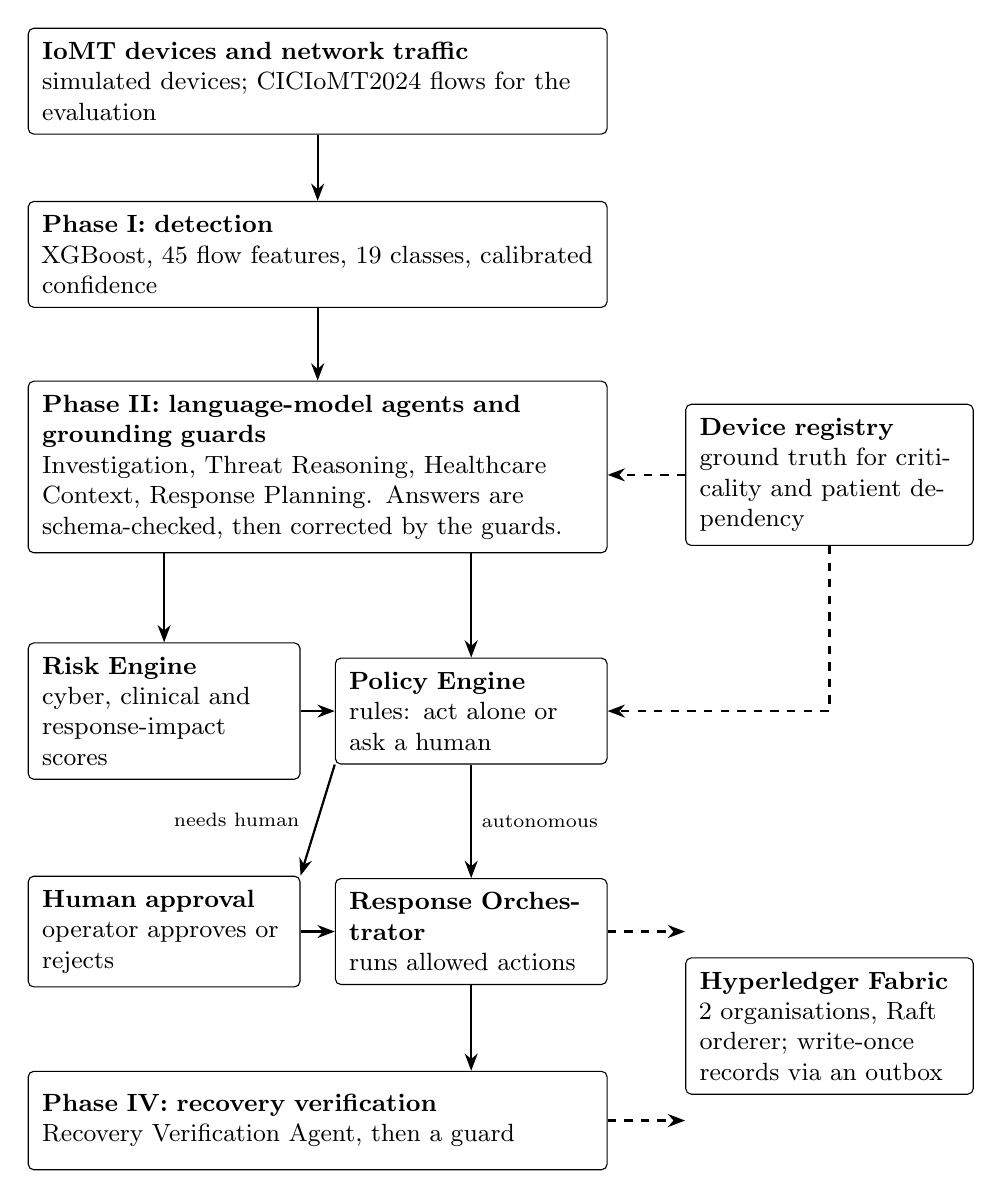
\begin{tikzpicture}[
  font=\small,
  box/.style={draw, rounded corners=2pt, align=left, inner sep=5pt, text width=7.0cm, minimum height=1.25cm},
  half/.style={box, text width=3.1cm},
  side/.style={box, text width=3.3cm},
  arr/.style={-{Stealth[length=2.2mm]}, thick},
  dsh/.style={arr, dashed}]
\node[box] (dev) at (0,0) {\textbf{IoMT devices and network traffic}\\ simulated devices; CICIoMT2024 flows for the evaluation};
\node[box] (det) at (0,-2.2) {\textbf{Phase I: detection}\\ XGBoost, 45 flow features, 19 classes, calibrated confidence};
\node[box] (ag) at (0,-4.9) {\textbf{Phase II: language-model agents and grounding guards}\\ Investigation, Threat Reasoning, Healthcare Context, Response Planning. Answers are schema-checked, then corrected by the guards.};
\node[half] (risk) at (-1.95,-8.0) {\textbf{Risk Engine}\\ cyber, clinical and response-impact scores};
\node[half] (pol) at (1.95,-8.0) {\textbf{Policy Engine}\\ rules: act alone or ask a human};
\node[half] (hum) at (-1.95,-10.8) {\textbf{Human approval}\\ operator approves or rejects};
\node[half] (resp) at (1.95,-10.8) {\textbf{Response Orchestrator}\\ runs allowed actions};
\node[box] (rec) at (0,-13.2) {\textbf{Phase IV: recovery verification}\\ Recovery Verification Agent, then a guard};
\node[side] (reg) at (6.5,-5.0) {\textbf{Device registry}\\ ground truth for criticality and patient dependency};
\node[side] (led) at (6.5,-12.0) {\textbf{Hyperledger Fabric}\\ 2 organisations, Raft orderer; write-once records via an outbox};
\draw[arr] (dev.south) -- (det.north);
\draw[arr] (det.south) -- (ag.north);
\draw[arr] (ag.south -| risk.north) -- (risk.north);
\draw[arr] (ag.south -| pol.north) -- (pol.north);
\draw[arr] (risk.east) -- (pol.west);
\draw[arr] (pol.south west) -- (hum.north east) node[midway, left, font=\scriptsize, xshift=-1mm] {needs human};
\draw[arr] (pol.south) -- (resp.north) node[midway, right, font=\scriptsize] {autonomous};
\draw[arr] (hum.east) -- (resp.west);
\draw[arr] (resp.south) -- (resp.south |- rec.north);
\draw[dsh] (reg.west) -- (reg.west -| ag.east);
\draw[dsh] (reg.south) |- (pol.east);
\draw[dsh] (resp.east) -- (resp.east -| led.west);
\draw[dsh] (rec.east) -- (rec.east -| led.west);
\end{tikzpicture}
\caption{Architecture of the proposed framework. Solid arrows: data and control flow. Dashed arrows: registry reads and ledger writes.}
\label{fig:arch}
\end{figure}

\subsection{Phases of the framework}
The framework runs in four phases (Figure~\ref{fig:phases}). Phase~I detects an attack and attaches a calibrated confidence. Phase~II lets the agents investigate and propose one action, with every answer checked by the guards. Phase~III scores the situation and decides, through the Policy Engine, whether the action runs alone or waits for a human. Phase~IV verifies the outcome and closes or reopens the incident. The ledger bar at the bottom of Figure~\ref{fig:phases} shows that the ledger is written at the end of Phases~I, III and~IV, and never sits on the path between a decision and its execution.

\begin{figure}[htbp]
\centering
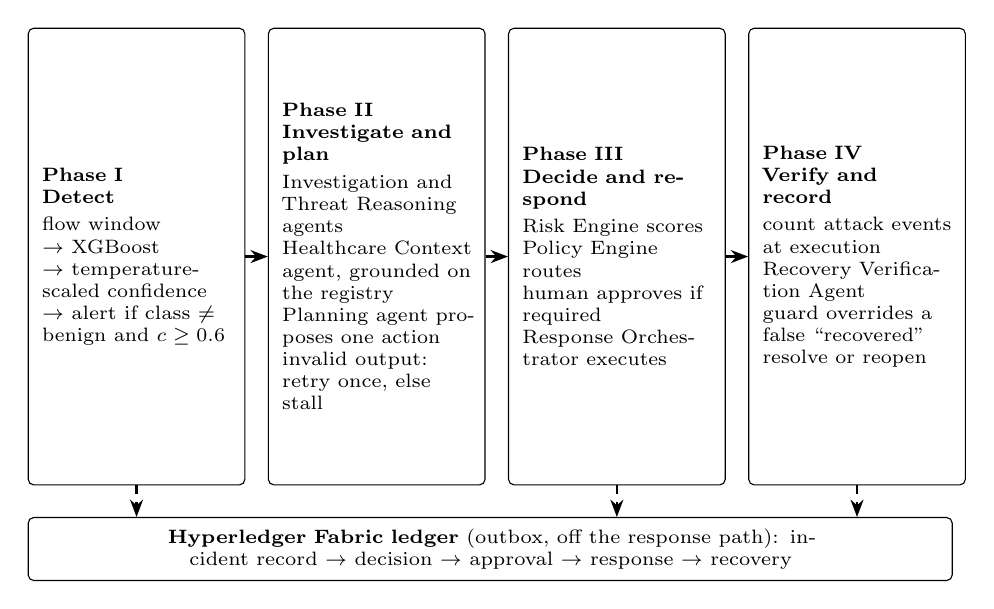
\begin{tikzpicture}[
  font=\scriptsize,
  ph/.style={draw, rounded corners=2pt, align=left, inner sep=5pt, text width=2.4cm, minimum height=5.8cm, anchor=north},
  arr/.style={-{Stealth[length=2.2mm]}, thick}]
\node[ph] (p1) at (0,0) {\textbf{Phase I\\ Detect}\\[2pt] flow window\\ $\rightarrow$ XGBoost\\ $\rightarrow$ temperature-scaled confidence\\ $\rightarrow$ alert if class $\neq$ benign and $c\ge 0.6$};
\node[ph] (p2) at (3.05,0) {\textbf{Phase II\\ Investigate and plan}\\[2pt] Investigation and Threat Reasoning agents\\ Healthcare Context agent, grounded on the registry\\ Planning agent proposes one action\\ invalid output: retry once, else stall};
\node[ph] (p3) at (6.1,0) {\textbf{Phase III\\ Decide and respond}\\[2pt] Risk Engine scores\\ Policy Engine routes\\ human approves if required\\ Response Orchestrator executes};
\node[ph] (p4) at (9.15,0) {\textbf{Phase IV\\ Verify and record}\\[2pt] count attack events at execution\\ Recovery Verification Agent\\ guard overrides a false ``recovered''\\ resolve or reopen};
\draw[arr] (p1.east) -- (p2.west);
\draw[arr] (p2.east) -- (p3.west);
\draw[arr] (p3.east) -- (p4.west);
\node[draw, rounded corners=2pt, text width=11.5cm, minimum height=0.8cm, anchor=north west, align=center, font=\scriptsize] (ledger) at ([yshift=-0.4cm]p1.south west) {\textbf{Hyperledger Fabric ledger} (outbox, off the response path): incident record $\rightarrow$ decision $\rightarrow$ approval $\rightarrow$ response $\rightarrow$ recovery};
\draw[arr, dashed] (p1.south) -- (p1.south |- ledger.north);
\draw[arr, dashed] (p3.south) -- (p3.south |- ledger.north);
\draw[arr, dashed] (p4.south) -- (p4.south |- ledger.north);
\end{tikzpicture}
\caption{The four phases of the framework and the points at which ledger records are written (dashed arrows).}
\label{fig:phases}
\end{figure}

\subsection{Phase I: detection and calibrated confidence}
A flow window with feature vector $\mathbf{x}$ is classified by an XGBoost model into one of $K=19$ classes (Benign plus 18 attack types). With logits $z_k(\mathbf{x})$, the calibrated probability and confidence are
\begin{equation}
p_k(\mathbf{x}) = \frac{\exp\!\big(z_k(\mathbf{x})/T\big)}{\sum_{j=1}^{K}\exp\!\big(z_j(\mathbf{x})/T\big)},\qquad c(\mathbf{x}) = \max_k p_k(\mathbf{x}),
\label{eq:temp}
\end{equation}
where the temperature $T$ is fitted by minimising the negative log-likelihood on a validation split ($T=0.917$ in our run). An alert is raised when the predicted class $\hat y$ is not Benign and $c\ge\theta$ with $\theta=0.6$. An optional \emph{confidence gate} additionally forbids autonomous action when $c<\tau$; $\tau$ is chosen on validation data only (Section~\ref{sec:gate}). Equation~\eqref{eq:temp} is the only place the temperature enters; it rescales confidence without changing which class has the largest probability.

\subsection{Phase II: guarded agents}
Five agents are used: Investigation, Threat Reasoning, Healthcare Context, Response Planning and Recovery Verification (the last in Phase~IV). Each returns JSON that must satisfy a schema. A parse or schema failure triggers one retry; a second failure stalls the incident in a safe state (for example \texttt{investigation\_stalled}) instead of guessing. Three deterministic guards then correct what the agents claim: the clinical-context guard, the recovery-claim guard and the incident-identity guard.
\begin{align}
\kappa' &= \kappa_{\mathrm{reg}}(d), \qquad \pi' = \pi_{\mathrm{reg}}(d), \label{eq:g1}\\
i' &= \max(i,\mathrm{HIGH}) \ \text{ if } \kappa_{\mathrm{reg}}(d)=\mathrm{HIGH}\wedge \pi_{\mathrm{reg}}(d), \label{eq:g1b}\\
\mathrm{success}' &= \mathrm{success}\wedge (n_{\mathrm{after}}\le n_{\mathrm{exec}}), \label{eq:g2}\\
\text{accept } o &\iff \mathrm{id}(o)=\mathrm{id}(\text{incident}). \label{eq:g3}
\end{align}
Equations~\eqref{eq:g1} and~\eqref{eq:g1b} define the clinical-context guard, Eq.~\eqref{eq:g2} the recovery-claim guard and Eq.~\eqref{eq:g3} the incident-identity guard.
In these equations $\kappa$ is device criticality, $\pi$ is patient dependency, $i$ is the stated clinical impact, $d$ is the device, $o$ is an agent's output, $n_{\mathrm{exec}}$ is the count of attack events observed when the action was executed and $n_{\mathrm{after}}$ the count at verification. The recovery-claim guard uses an event count, not a clock, so it needs no synchronised time. Every correction is logged and stored in the incident trace next to the agent's original output.

\subsection{Phase III: Risk Engine and Policy Engine}
\label{sec:phase3}
The Risk Engine is an explicit rule table, not a learned model, so each score can be audited. With threat severity $s$ and the Threat Reasoning Agent's confidence $\gamma\in[0,1]$, device criticality $\kappa$, clinical impact $i$ and patient dependency $\pi\in\{0,1\}$:
\begin{align}
R_{\mathrm{cyber}} &= b_s\,(0.5+0.5\,\gamma),\label{eq:cyber}\\
R_{\mathrm{clin}} &= \min\{1,\ \max(b_\kappa+\Delta_i,\ 0.55\,\pi)\}.\label{eq:clin}
\end{align}
The base scores are $b_s\in\{0.15,0.40,0.70,0.90\}$ for low, medium, high and critical severity, $b_\kappa\in\{0.10,0.35,0.60\}$ for low, medium and high criticality, and $\Delta_i\in\{0,0.05,0.15,0.25\}$ for low to critical clinical impact.
The 0.5 floor in~\eqref{eq:cyber} stops a low-confidence severe assessment from scoring near zero, and the 0.55 floor in~\eqref{eq:clin} means a device a patient depends on never scores low clinical risk. The third score, \emph{response impact}, says how harmful the \emph{action itself} would be on this device. Table~\ref{tab:impact} gives its values: the same severe action is rated medium impact on a device without a patient, high on a patient-dependent device and critical on a high-criticality, patient-dependent device.

\begin{table}[htbp]
\centering
\caption{Response impact of an action, by its disruption tier and the device context.}
\label{tab:impact}
\small
\begin{tabular}{@{}L{5.0cm}C{2.8cm}C{2.4cm}C{2.4cm}@{}}
\toprule
Action tier (examples) & HIGH criticality and patient-dependent & Patient-dependent & Not patient-dependent \\
\midrule
Severe: shutdown, isolate critical, quarantine segment, failover & Critical & High & Medium \\
Moderate: isolate non-critical, restrict communication, restart service, block traffic & High & Medium & Low \\
Non-disruptive: rotate credentials, revoke session, activate backup & Medium & Low & Low \\
\bottomrule
\end{tabular}
\end{table}

The Policy Engine routes the single action the planner recommends, and the first matching rule wins. A patient-dependent device with a severe action of shutdown or critical isolation always goes to a human. Otherwise an action whose response impact is low or less runs autonomously; a medium impact runs autonomously if the device is not patient-dependent and goes to a human if it is (a conservative gap-filling rule); and a high or critical impact always goes to a human. No rule reads a model's opinion of the device or the attack. The optional confidence gate of Section~\ref{sec:gate} is checked last and can only turn an autonomous decision into a human one, never the reverse. Each decision carries a stable rule identifier so a reviewer can see which rule fired, and Section~\ref{sec:exhaustive} checks these rules over their entire input space.

\subsection{Phase IV: recovery verification and provenance}
After an action runs, the system records $n_{\mathrm{exec}}$, the Recovery Verification Agent judges whether the device is safe, and the recovery-claim guard overrides a success claim if attack events have continued. A failed check reopens the incident. Five write-once records go to Hyperledger Fabric 2.5.9: the incident, decision, approval, response and recovery records. Each stores an evidence hash rather than the evidence. A transaction commits only if a majority of the two organisations (Hospital and SecurityOps) endorse it, and the client waits for both peers' commit events before reporting success. A verification function recomputes a hash and checks that it is on the ledger.

\subsection{Algorithms}
Algorithm~\ref{alg:main} is the end-to-end procedure for one flow window. Algorithm~\ref{alg:guard} is the guarded agent call used inside it. The detector runs on every flow window, but only an alert opens an incident, so the agents, engines and ledger run at incident rate, not flow rate. Because the engines and guards are plain code, they can be unit-tested exhaustively; the language-model calls are the only non-deterministic step, and a failure there stalls safely or is corrected, never executed. The implementation is a Python backend with FastAPI, XGBoost for the detector, a Node.js chaincode for Fabric, and a simulated hospital of devices for the response and recovery steps.

\begin{algorithm}[htbp]
\caption{Incident handling in the proposed framework}
\label{alg:main}
\begin{algorithmic}[1]
\Require flow window $\mathbf{x}$ on device $d$; registry $\mathcal{R}$; thresholds $\theta$, optional $\tau$
\State $(\hat y, c)\gets \textsc{Detect}(\mathbf{x})$ \Comment{Eq.~\eqref{eq:temp}}
\If{$\hat y=\text{Benign}$ \textbf{or} $c<\theta$}
  \State \Return
\EndIf
\State open incident $u$ and call \textsc{Ledger.recordIncident}$(u)$
\State $E\gets \textsc{GuardedCall}(\text{Investigation}, u)$
\State $A\gets \textsc{GuardedCall}(\text{ThreatReasoning}, E)$
\State $C\gets \textsc{GuardedCall}(\text{HealthcareContext}, u)$
\State $C\gets \textsc{ContextGuard}(C,\mathcal{R}[d])$ \Comment{Eqs.~\eqref{eq:g1}, \eqref{eq:g1b}}
\State $P\gets \textsc{GuardedCall}(\text{ResponsePlanning}, A, C)$
\State $a\gets P.\text{recommended}$
\State $S\gets \textsc{RiskEngine}(A, C, P)$ \Comment{Eqs.~\eqref{eq:cyber}, \eqref{eq:clin}; Table~\ref{tab:impact}}
\State $(h, \rho)\gets \textsc{PolicyEngine}(S, C, a, c, \tau)$ \Comment{rules of Section~\ref{sec:phase3}}
\State \textsc{Ledger.recordDecision}$(u, a, \rho)$
\If{$h$}
  \State wait for the operator; \textsc{Ledger.recordApproval}$(u)$
  \If{rejected} \State \Return \EndIf
\EndIf
\State $n_{\mathrm{exec}}\gets \textsc{CountAttackEvents}(d)$
\State execute $a$ and call \textsc{Ledger.recordResponse}$(u)$
\State $V\gets \textsc{GuardedCall}(\text{RecoveryVerification}, u)$
\State $V\gets \textsc{RecoveryGuard}(V, n_{\mathrm{exec}})$ \Comment{Eq.~\eqref{eq:g2}}
\State \textsc{Ledger.recordRecovery}$(u)$
\State mark $u$ resolved if $V.\text{success}$, otherwise reopened
\end{algorithmic}
\end{algorithm}

\begin{algorithm}[htbp]
\caption{\textsc{GuardedCall}: schema validation, retry and identity check}
\label{alg:guard}
\begin{algorithmic}[1]
\Require agent $g$, prompt $q$, schema $\Sigma$, incident id $u$
\For{$attempt=1,2$}
  \State $o\gets \textsc{LLM}(g,q)$
  \If{$o$ parses, satisfies $\Sigma$ and $\mathrm{id}(o)=u$} \Comment{incident-identity guard, Eq.~\eqref{eq:g3}}
    \State \Return $o$
  \EndIf
\EndFor
\State stall the incident safely (no action is taken)
\end{algorithmic}
\end{algorithm}

Algorithm~\ref{alg:main} shows where each earlier component sits: the detector (line 1) uses Eq.~\eqref{eq:temp}, the clinical-context guard (line 8) corrects the Healthcare Context Agent before anything is scored, and the Risk and Policy engines (lines 11--12) see only corrected inputs. The ledger calls are plain writes between steps. In Algorithm~\ref{alg:guard} the only way out of the loop other than a valid answer is a safe stall, which is why a model that returns garbage, or an answer about the wrong incident, cannot cause an action.

%% ==========================================================================
\section{Results}
\label{sec:results}

\subsection{Experimental setup}
\label{sec:setup}
The evaluation has eight parts, each answering one question about one part of the framework. The detector is measured on real data (Sections~\ref{sec:detector} and~\ref{sec:robust}); its confidence and the confidence gate are checked (Section~\ref{sec:gate}); the patient-safety behaviour of the decision layer is measured against baselines and ablations (Section~\ref{sec:safety}) and stress-tested over different clinical device mixes (Section~\ref{sec:sensitivity}); the decision rules are verified over their whole input space (Section~\ref{sec:exhaustive}); the agentic layer is attacked with injected faults (Section~\ref{sec:agents}); and the blockchain is measured on a real Fabric network (Section~\ref{sec:chain}). Every figure and table below is produced by a script in the project repository and written to a report file; none is typed by hand. The repository is available on request from the authors (TODO: add the public repository link).

The backend is Python (FastAPI) with an XGBoost detector (150 trees, depth 8, learning rate 0.2, histogram method, 256 bins) and a random-forest comparator (100 trees). Fabric 2.5.9 runs natively on one host with 2 CPUs: two organisations (Hospital, SecurityOps) with one peer each, one Raft orderer with a 1~s batch timeout, a Node.js chaincode through an external builder, and a majority endorsement policy. Detector training uses fixed seeds (seed 42 for the main model; seeds 0--4 for the multi-seed study) and the device-context sampling of the safety study uses five fixed seeds.

\subsection{Dataset}
\label{sec:dataset}
We use the WiFi and MQTT release of CICIoMT2024~\cite{dadkhah2024}, a benchmark of network flows from a testbed of IoMT devices under attack. MQTT (Message Queuing Telemetry Transport) is a publish-subscribe protocol widely used by medical sensors. The attacks fall into six families: MQTT attacks (floods and malformed data), reconnaissance scans, ARP spoofing, and TCP/IP denial-of-service (DoS) and distributed denial-of-service (DDoS) floods over ICMP, SYN, TCP and UDP. The official capture-level split is kept: no random re-splitting and no tuning on the test split. Table~\ref{tab:dataset} gives the dimensions. The test split is dominated by volumetric floods (about 1.5 million of its 1.6 million flows), so overall accuracy is high by construction and macro-F1, which weights all 19 classes equally, is the more informative figure.

\begin{table}[htbp]
\centering
\caption{CICIoMT2024 (WiFi and MQTT) as used in this work.}
\label{tab:dataset}
\small
\begin{tabular}{@{}L{5.0cm}L{7.5cm}@{}}
\toprule
Property & Value \\
\midrule
Official training rows & 7,017,530 (training capped at 300,000 per class for the main XGBoost model, 30,000 for the main random forest) \\
Rows used by the main models & 2,975,443 (XGBoost); 441,318 (random forest) \\
Official test rows (all used, none sampled) & 1,614,182: 37,607 benign, 1,576,575 attack \\
Features per flow & 45 (the dataset's own flow features) \\
Classes & 19: Benign and 18 attacks (MQTT floods and malformed data; TCP/IP DDoS and DoS; reconnaissance; ARP spoofing) \\
Clinical device context & Not in the dataset; simulated (Section~\ref{sec:safety}) \\
\bottomrule
\end{tabular}
\end{table}

Table~\ref{tab:dataset} also shows the main limit of the data for our purpose: the files describe network flows only, so which device was attacked, how critical it is and whether a patient depends on it must be supplied separately. Sections~\ref{sec:safety} and~\ref{sec:sensitivity} do this by sampling, and say so wherever it matters.

\subsection{Evaluation metrics}
\label{sec:metrics}
For the detector we report accuracy, macro-F1 (the unweighted mean of per-class F1 over 19 classes, or over six attack families), the attack-detection rate (the share of attack flows flagged as any attack), the benign false-positive rate (the share of benign flows flagged as an attack), the area under the ROC curve (AUC) and average precision for attack versus benign, the expected calibration error (ECE, the confidence-weighted gap between stated confidence and observed accuracy over 15 equal-width bins) and the negative log-likelihood (NLL).

For safety we define three rates. The \emph{unsafe autonomous action rate} is, among real attacks that hit a HIGH-criticality, patient-dependent device (the high-stakes trials), the share for which the system executed a disruptive action with no human approval. The \emph{unnecessary isolation rate} is, among detector false positives (benign flows flagged as attacks), the share for which the system autonomously isolated the device anyway. \emph{Autonomy retained} is the share of fired detections that the system handles without a human. We always report these rates together with their counts, because a rate of zero means something different when the denominator is 10 than when it is 262,000. For the ledger we report integrity-check outcomes, latency percentiles and committed throughput.

\subsection{Detector performance}
\label{sec:detector}
Table~\ref{tab:detector} reports the two main detectors on the entire test split. XGBoost reaches 99.52\% 19-class accuracy, macro-F1 0.9263 and 99.97\% attack detection, with a benign false-positive rate of 5.09\% at the arg-max operating point. At the runtime operating point (alert only when confidence is at least 0.6) attack detection is 99.72\% and the benign false-positive rate falls to 3.12\% (1,174 of 37,607 benign flows flagged). Of the 1,576,575 attack flows, XGBoost misses 440 as binary decisions (true positives 1,576,135; false positives 1,916; true negatives 35,691; precision 0.9988). Random forest is weaker on macro-F1 (0.8704) and has a higher benign false-positive rate (6.73\%), but trains in 56~s against 749~s.

\begin{table}[htbp]
\centering
\caption{Detector results on the full CICIoMT2024 test split (1,614,182 flows), main models trained once with seed 42.}
\label{tab:detector}
\footnotesize
\begin{tabular}{@{}l@{\hspace{6pt}}c@{\hspace{5pt}}c@{\hspace{5pt}}c@{\hspace{5pt}}c@{\hspace{5pt}}c@{\hspace{5pt}}c@{}}
\toprule
Model & Acc.\ (19) & F1$_{\mathrm{macro}}$ (19) & F1$_{\mathrm{macro}}$ (6) & Attack det. & Benign FPR & Train (s) \\
\midrule
XGBoost & 0.9952 & 0.9263 & 0.9126 & 0.9997 & 0.0509 & 749 \\
Random forest & 0.9916 & 0.8704 & 0.9036 & 0.9995 & 0.0673 & 56 \\
\bottomrule
\end{tabular}
\end{table}

Figure~\ref{fig:f1} shows the per-class F1 of XGBoost. The volumetric classes are near perfect (F1 above 0.99 for the DDoS and DoS TCP/IP classes). The weak classes are ARP spoofing (F1 0.5346, precision 0.4055) and vulnerability scanning (0.6919); both are rare in the data. This matters downstream: 94.4\% of the detector's false alarms are predicted as ARP spoofing, so the weakness is concentrated in one class.

\begin{figure}[htbp]
\centering
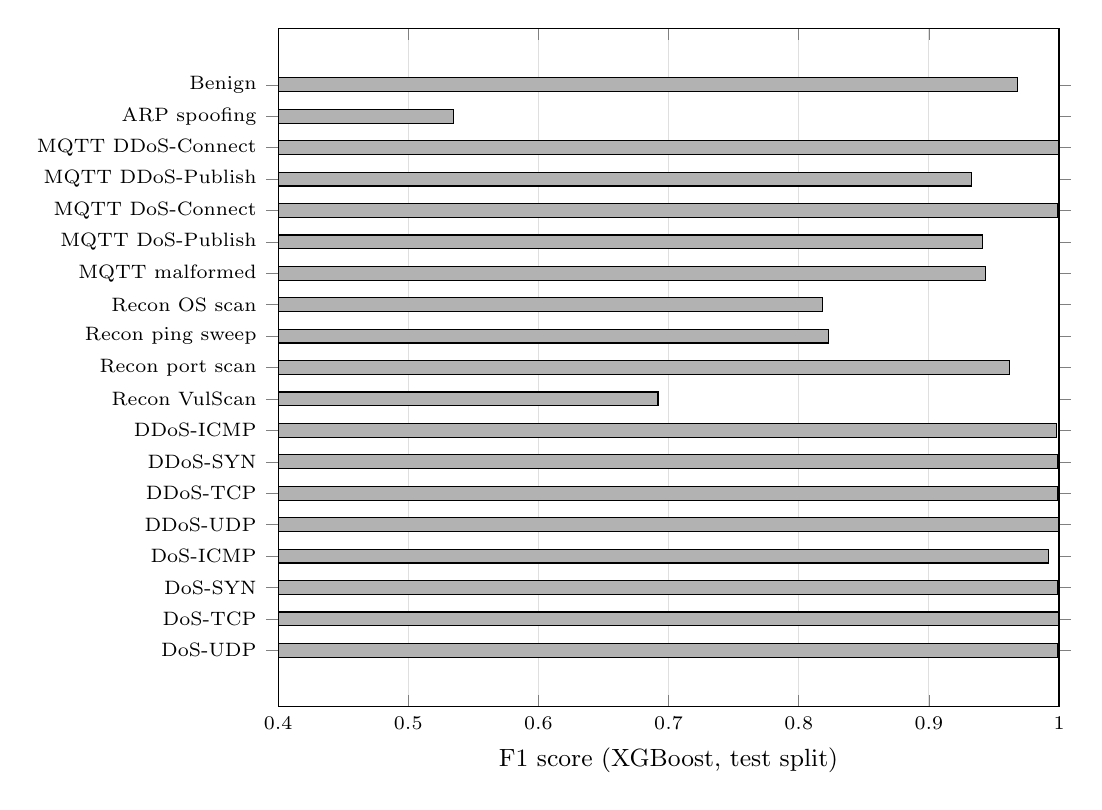
\begin{tikzpicture}
\begin{axis}[
  xbar, width=11.5cm, height=10.2cm, bar width=5pt,
  xmin=0.4, xmax=1.0, xlabel={F1 score (XGBoost, test split)},
  symbolic y coords={Benign,ARP spoofing,MQTT DDoS-Connect,MQTT DDoS-Publish,MQTT DoS-Connect,MQTT DoS-Publish,MQTT malformed,Recon OS scan,Recon ping sweep,Recon port scan,Recon VulScan,DDoS-ICMP,DDoS-SYN,DDoS-TCP,DDoS-UDP,DoS-ICMP,DoS-SYN,DoS-TCP,DoS-UDP},
  ytick=data, y dir=reverse, yticklabel style={font=\scriptsize},
  xmajorgrids, grid style={gray!25}, tick label style={font=\scriptsize}, label style={font=\small}]
\addplot[fill=gray!60, draw=black] coordinates {
 (0.9680,Benign) (0.5346,ARP spoofing) (0.9999,MQTT DDoS-Connect) (0.9326,MQTT DDoS-Publish)
 (0.9990,MQTT DoS-Connect) (0.9415,MQTT DoS-Publish) (0.9437,MQTT malformed) (0.8184,Recon OS scan)
 (0.8229,Recon ping sweep) (0.9617,Recon port scan) (0.6919,Recon VulScan) (0.9978,DDoS-ICMP)
 (0.9992,DDoS-SYN) (0.9992,DDoS-TCP) (0.9994,DDoS-UDP) (0.9916,DoS-ICMP) (0.9992,DoS-SYN)
 (0.9995,DoS-TCP) (0.9990,DoS-UDP)};
\end{axis}
\end{tikzpicture}
\caption{Per-class F1 of the XGBoost detector on the full test split (macro-F1 0.9263). ARP spoofing and vulnerability scanning are the weak classes.}
\label{fig:f1}
\end{figure}

Because the dataset rows carry no wall-clock timestamp, detection delay is counted in flows. On all 20 attack captures in the test split the detector's first alert came at flow 0 (17 captures) or flow 1 (3 captures), and every capture was alerted within its first 10 flows. The share of a capture's flows that raised an alert ranged from 73.6\% (vulnerability scanning) to 100\%.

\subsection{Robustness of the detector: seeds, classifiers and uncertainty}
\label{sec:robust}
A single trained model, as in Table~\ref{tab:detector}, cannot show how much of a difference between two classifiers is training noise, and a single accuracy figure hides where the errors are. This section therefore repeats the detector study with more classifiers and seeds, adds confidence intervals, and examines the errors.

Table~\ref{tab:multiseed} trains six classifiers five times each. A training seed changes both the random sample of at most 30,000 training flows per class and the model's own randomness; every model is scored on the entire test split. The smaller training cap (30,000 instead of 300,000 flows per class) makes thirty trainings affordable on a 2-CPU machine, so the XGBoost row is not the same model as in Table~\ref{tab:detector}. The decision tree, random forest, extra-trees and XGBoost models are scale-free; the logistic regression (trained by stochastic gradient descent) and the neural network (one hidden layer of 64 units) receive log-scaled and standardised features, because the raw features are heavy-tailed. The linear and neural baselines were not tuned.

\begin{table}[htbp]
\centering
\caption{Six classifiers on the full test split: mean $\pm$ sample standard deviation over training seeds. Each model is trained on at most 30,000 flows per class.}
\label{tab:multiseed}
\footnotesize
\resizebox{\textwidth}{!}{\begin{tabular}{@{}lcccccc@{}}
\toprule
Classifier & Seeds & Accuracy (19) & Macro-F1 (19) & Attack detection & Benign FPR & Train (s) \\
\midrule
Decision tree & 5 & 0.9950 $\pm$ 0.0003 & 0.9080 $\pm$ 0.0051 & 0.9996 $\pm$ 0.0000 & 0.0857 $\pm$ 0.0037 & 8 \\
Logistic regression (SGD) & 5 & 0.6200 $\pm$ 0.0296 & 0.5690 $\pm$ 0.0084 & 0.9993 $\pm$ 0.0001 & 0.1902 $\pm$ 0.0054 & 69 \\
Random forest & 5 & 0.9922 $\pm$ 0.0010 & 0.8783 $\pm$ 0.0131 & 0.9993 $\pm$ 0.0000 & 0.0499 $\pm$ 0.0107 & 50 \\
Extra trees & 5 & 0.9896 $\pm$ 0.0001 & 0.8600 $\pm$ 0.0011 & 0.9994 $\pm$ 0.0000 & 0.0604 $\pm$ 0.0026 & 23 \\
Neural network (1 hidden layer) & 5 & 0.6883 $\pm$ 0.0389 & 0.6616 $\pm$ 0.0099 & 0.9994 $\pm$ 0.0002 & 0.1303 $\pm$ 0.0386 & 55 \\
XGBoost & 5 & 0.9953 $\pm$ 0.0002 & 0.9103 $\pm$ 0.0017 & 0.9997 $\pm$ 0.0000 & 0.0671 $\pm$ 0.0078 & 88 \\
\bottomrule
\end{tabular}}
\end{table}


Table~\ref{tab:multiseed} shows three things. First, the tree-based models form a cluster: the decision tree, random forest, extra trees and XGBoost reach between 0.9896 and 0.9953 accuracy, and XGBoost has the highest accuracy (0.9953) and macro-F1 (0.9103) and the smallest spread over seeds (standard deviations 0.0002 and 0.0017). Second, the margin between XGBoost and a single decision tree is small: 0.0003 in accuracy and 0.0023 in macro-F1, about half the tree's seed-to-seed standard deviation of 0.0051. On this dataset the choice of XGBoost over a simpler tree is therefore supported by its stability and not by a large gain, and we do not claim otherwise. Third, the linear and neural baselines are far weaker (accuracy 0.62 and 0.69, macro-F1 0.57 and 0.66), which suggests that the classes are separated by sharp thresholds on individual features, such as protocol flags and rates, that a linear boundary or a small untuned network does not capture. Across all six classifiers the attack-detection rate stays between 0.9993 and 0.9997; what varies is the benign false-positive rate (0.050 to 0.190) and macro-F1. With 30,000 training flows per class XGBoost reaches the same accuracy as the main model trained on up to 300,000 (0.9953 against 0.9952) but a lower macro-F1 (0.9103 against 0.9263) and a higher benign false-positive rate (0.067 against 0.051), so the larger training cap helps the rare classes.


Table~\ref{tab:boot} gives 95\% bootstrap intervals for the main XGBoost model of Table~\ref{tab:detector}, obtained by resampling the test flows 1,000 times. The intervals are narrow (accuracy 0.9951--0.9953; macro-F1 0.9233--0.9291), but they treat the 1.6 million flows as independent. Flows inside one capture are strongly correlated, so these intervals understate the uncertainty across captures and should be read as a lower bound on it; the spread across training seeds in Table~\ref{tab:multiseed} is the more honest guide.

\begin{table}[htbp]
\centering
\caption{Main XGBoost model on the full test split: point estimates and 95\% bootstrap intervals (1,000 resamples).}
\label{tab:boot}
\small
\begin{tabular}{@{}L{4.2cm}C{2.4cm}C{4.2cm}@{}}
\toprule
Metric & Estimate & 95\% interval \\
\midrule
Accuracy (19 classes) & 0.9952 & 0.9951 -- 0.9953 \\
Macro-F1 (19 classes) & 0.9263 & 0.9233 -- 0.9291 \\
Attack-detection rate & 0.9997 & 0.99970 -- 0.99975 \\
Benign false-positive rate & 0.0509 & 0.0489 -- 0.0533 \\
\bottomrule
\end{tabular}
\end{table}

Where the errors are is shown in Table~\ref{tab:family} and Figure~\ref{fig:confusion}. At the level of attack families, almost all errors are between DoS and DDoS (470 DoS flows predicted as DDoS and 1,646 the other way) and between benign traffic and ARP spoofing or reconnaissance. The largest single confusions in Figure~\ref{fig:confusion} are benign flows predicted as ARP spoofing (1,631), TCP/IP DDoS-ICMP predicted as DoS-ICMP (1,309), MQTT DDoS-Publish predicted as DoS-Publish (1,056), and port scans confused with operating-system scans (582 and 463). These are pairs whose traffic differs mainly in the number of attacking sources, which a per-flow feature vector cannot see. For the present purpose they are cheap errors: the response of the framework depends on whether a flow is an attack, and not on which attack it is, so confusing a DoS with a DDoS changes no decision. The costly errors are the 1,631 benign flows flagged as ARP spoofing and the 440 attack flows predicted as benign.

\begin{table}[htbp]
\centering
\caption{Confusion between the six attack families on the full test split (rows: true family; columns: predicted family).}
\label{tab:family}
\scriptsize
\setlength{\tabcolsep}{3pt}
\begin{tabular}{@{}lrrrrrrrr@{}}
\toprule
True family & Flows & Benign & ARP spoof. & MQTT & Recon & DoS & DDoS & Recall \\
\midrule
Benign & 37,607 & 35,691 & 1,631 & 25 & 260 & 0 & 0 & 0.9491 \\
ARP spoofing & 1,744 & 106 & 1,368 & 4 & 266 & 0 & 0 & 0.7844 \\
MQTT & 63,715 & 54 & 45 & 63,602 & 14 & 0 & 0 & 0.9982 \\
Recon & 27,676 & 273 & 289 & 34 & 27,079 & 1 & 0 & 0.9784 \\
DoS & 416,676 & 1 & 1 & 4 & 4 & 416,196 & 470 & 0.9988 \\
DDoS & 1,066,764 & 6 & 40 & 26 & 82 & 1,646 & 1,064,964 & 0.9983 \\
\bottomrule
\end{tabular}
\end{table}


\begin{figure}[htbp]
\centering
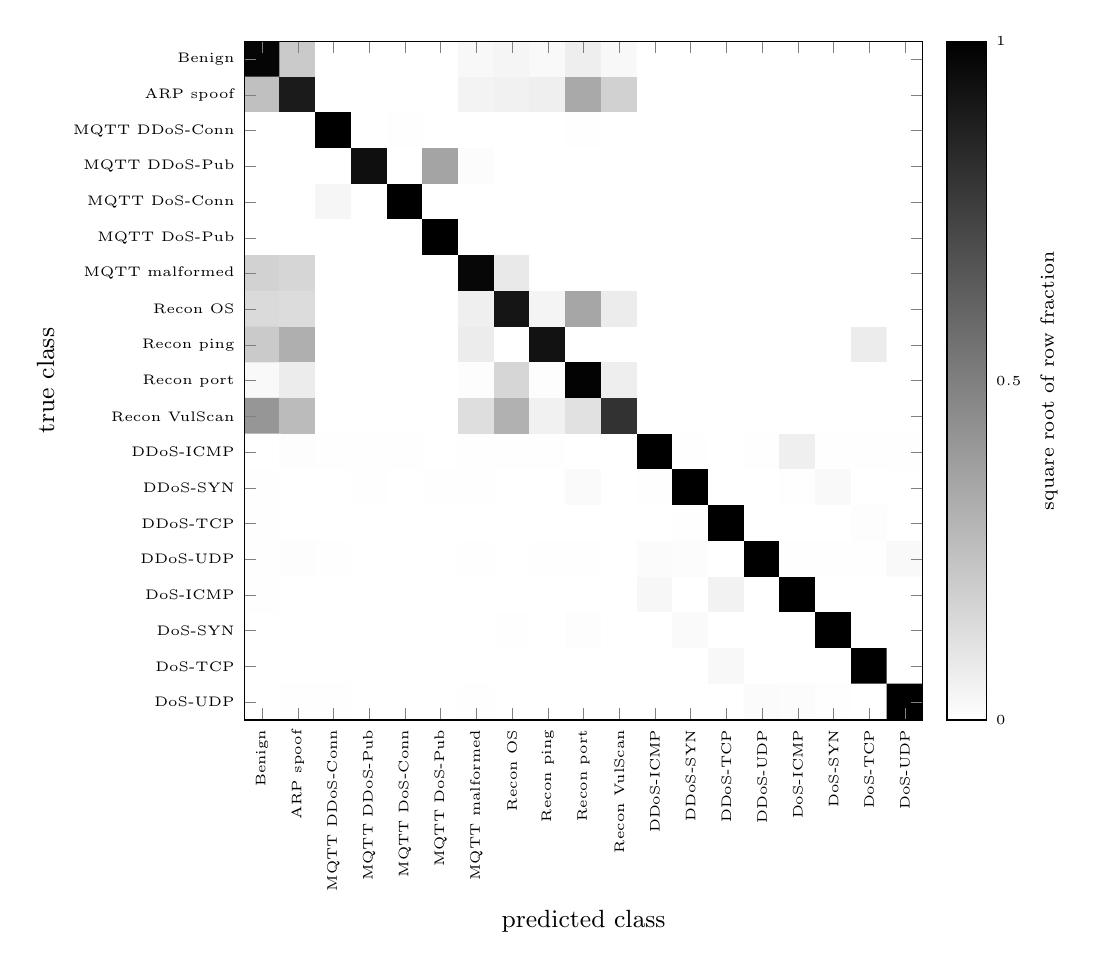
\begin{tikzpicture}
\begin{axis}[
  width=10.2cm, height=10.2cm, enlarge x limits=false, enlarge y limits=false,
  axis on top, y dir=reverse, xlabel={predicted class}, ylabel={true class},
  xtick={0,1,2,3,4,5,6,7,8,9,10,11,12,13,14,15,16,17,18}, xticklabels={{Benign},{ARP spoof},{MQTT DDoS-Conn},{MQTT DDoS-Pub},{MQTT DoS-Conn},{MQTT DoS-Pub},{MQTT malformed},{Recon OS},{Recon ping},{Recon port},{Recon VulScan},{DDoS-ICMP},{DDoS-SYN},{DDoS-TCP},{DDoS-UDP},{DoS-ICMP},{DoS-SYN},{DoS-TCP},{DoS-UDP}}, xticklabel style={rotate=90, font=\tiny, anchor=east},
  ytick={0,1,2,3,4,5,6,7,8,9,10,11,12,13,14,15,16,17,18}, yticklabels={{Benign},{ARP spoof},{MQTT DDoS-Conn},{MQTT DDoS-Pub},{MQTT DoS-Conn},{MQTT DoS-Pub},{MQTT malformed},{Recon OS},{Recon ping},{Recon port},{Recon VulScan},{DDoS-ICMP},{DDoS-SYN},{DDoS-TCP},{DDoS-UDP},{DoS-ICMP},{DoS-SYN},{DoS-TCP},{DoS-UDP}}, yticklabel style={font=\tiny},
  colormap={wb}{color(0cm)=(white); color(1cm)=(black)},
  colorbar, colorbar style={ylabel={\scriptsize square root of row fraction}, ytick={0,0.5,1}, yticklabel style={font=\tiny}},
  point meta min=0, point meta max=1, tick label style={font=\tiny}, label style={font=\small}]
\addplot[matrix plot*, mesh/cols=19, point meta=explicit, draw=none] table[row sep=\\, x index=0, y index=1, meta index=2] {
0 0 0.974 \\
1 0 0.208 \\
2 0 0.000 \\
3 0 0.000 \\
4 0 0.000 \\
5 0 0.000 \\
6 0 0.026 \\
7 0 0.038 \\
8 0 0.022 \\
9 0 0.065 \\
10 0 0.028 \\
11 0 0.000 \\
12 0 0.000 \\
13 0 0.000 \\
14 0 0.000 \\
15 0 0.000 \\
16 0 0.000 \\
17 0 0.000 \\
18 0 0.000 \\
0 1 0.247 \\
1 1 0.886 \\
2 1 0.000 \\
3 1 0.000 \\
4 1 0.000 \\
5 1 0.000 \\
6 1 0.048 \\
7 1 0.054 \\
8 1 0.063 \\
9 1 0.336 \\
10 1 0.181 \\
11 1 0.000 \\
12 1 0.000 \\
13 1 0.000 \\
14 1 0.000 \\
15 1 0.000 \\
16 1 0.000 \\
17 1 0.000 \\
18 1 0.000 \\
0 2 0.000 \\
1 2 0.000 \\
2 2 1.000 \\
3 2 0.000 \\
4 2 0.005 \\
5 2 0.000 \\
6 2 0.000 \\
7 2 0.000 \\
8 2 0.000 \\
9 2 0.005 \\
10 2 0.000 \\
11 2 0.000 \\
12 2 0.000 \\
13 2 0.000 \\
14 2 0.000 \\
15 2 0.000 \\
16 2 0.000 \\
17 2 0.000 \\
18 2 0.000 \\
0 3 0.000 \\
1 3 0.000 \\
2 3 0.000 \\
3 3 0.935 \\
4 3 0.000 \\
5 3 0.354 \\
6 3 0.011 \\
7 3 0.000 \\
8 3 0.000 \\
9 3 0.000 \\
10 3 0.000 \\
11 3 0.000 \\
12 3 0.000 \\
13 3 0.000 \\
14 3 0.000 \\
15 3 0.000 \\
16 3 0.000 \\
17 3 0.000 \\
18 3 0.000 \\
0 4 0.000 \\
1 4 0.000 \\
2 4 0.036 \\
3 4 0.000 \\
4 4 0.999 \\
5 4 0.000 \\
6 4 0.000 \\
7 4 0.000 \\
8 4 0.000 \\
9 4 0.000 \\
10 4 0.000 \\
11 4 0.000 \\
12 4 0.000 \\
13 4 0.000 \\
14 4 0.000 \\
15 4 0.000 \\
16 4 0.000 \\
17 4 0.000 \\
18 4 0.000 \\
0 5 0.000 \\
1 5 0.000 \\
2 5 0.000 \\
3 5 0.000 \\
4 5 0.000 \\
5 5 1.000 \\
6 5 0.000 \\
7 5 0.000 \\
8 5 0.000 \\
9 5 0.000 \\
10 5 0.000 \\
11 5 0.000 \\
12 5 0.000 \\
13 5 0.000 \\
14 5 0.000 \\
15 5 0.000 \\
16 5 0.000 \\
17 5 0.000 \\
18 5 0.000 \\
0 6 0.176 \\
1 6 0.160 \\
2 6 0.000 \\
3 6 0.000 \\
4 6 0.000 \\
5 6 0.000 \\
6 6 0.967 \\
7 6 0.086 \\
8 6 0.000 \\
9 6 0.000 \\
10 6 0.000 \\
11 6 0.000 \\
12 6 0.000 \\
13 6 0.000 \\
14 6 0.000 \\
15 6 0.000 \\
16 6 0.000 \\
17 6 0.000 \\
18 6 0.000 \\
0 7 0.143 \\
1 7 0.138 \\
2 7 0.000 \\
3 7 0.000 \\
4 7 0.000 \\
5 7 0.000 \\
6 7 0.063 \\
7 7 0.910 \\
8 7 0.043 \\
9 7 0.348 \\
10 7 0.074 \\
11 7 0.000 \\
12 7 0.000 \\
13 7 0.000 \\
14 7 0.000 \\
15 7 0.000 \\
16 7 0.000 \\
17 7 0.000 \\
18 7 0.000 \\
0 8 0.207 \\
1 8 0.311 \\
2 8 0.000 \\
3 8 0.000 \\
4 8 0.000 \\
5 8 0.000 \\
6 8 0.073 \\
7 8 0.000 \\
8 8 0.922 \\
9 8 0.000 \\
10 8 0.000 \\
11 8 0.000 \\
12 8 0.000 \\
13 8 0.000 \\
14 8 0.000 \\
15 8 0.000 \\
16 8 0.000 \\
17 8 0.073 \\
18 8 0.000 \\
0 9 0.024 \\
1 9 0.074 \\
2 9 0.000 \\
3 9 0.000 \\
4 9 0.000 \\
5 9 0.000 \\
6 9 0.007 \\
7 9 0.160 \\
8 9 0.009 \\
9 9 0.982 \\
10 9 0.066 \\
11 9 0.000 \\
12 9 0.000 \\
13 9 0.000 \\
14 9 0.000 \\
15 9 0.000 \\
16 9 0.000 \\
17 9 0.000 \\
18 9 0.000 \\
0 10 0.410 \\
1 10 0.266 \\
2 10 0.000 \\
3 10 0.000 \\
4 10 0.000 \\
5 10 0.000 \\
6 10 0.128 \\
7 10 0.305 \\
8 10 0.054 \\
9 10 0.116 \\
10 10 0.797 \\
11 10 0.000 \\
12 10 0.000 \\
13 10 0.000 \\
14 10 0.000 \\
15 10 0.000 \\
16 10 0.000 \\
17 10 0.000 \\
18 10 0.000 \\
0 11 0.000 \\
1 11 0.008 \\
2 11 0.002 \\
3 11 0.002 \\
4 11 0.002 \\
5 11 0.000 \\
6 11 0.004 \\
7 11 0.002 \\
8 11 0.002 \\
9 11 0.000 \\
10 11 0.000 \\
11 11 0.998 \\
12 11 0.002 \\
13 11 0.000 \\
14 11 0.002 \\
15 11 0.061 \\
16 11 0.003 \\
17 11 0.002 \\
18 11 0.002 \\
0 12 0.003 \\
1 12 0.000 \\
2 12 0.000 \\
3 12 0.005 \\
4 12 0.000 \\
5 12 0.002 \\
6 12 0.004 \\
7 12 0.000 \\
8 12 0.000 \\
9 12 0.021 \\
10 12 0.000 \\
11 12 0.002 \\
12 12 0.999 \\
13 12 0.000 \\
14 12 0.000 \\
15 12 0.002 \\
16 12 0.024 \\
17 12 0.000 \\
18 12 0.000 \\
0 13 0.002 \\
1 13 0.000 \\
2 13 0.000 \\
3 13 0.000 \\
4 13 0.000 \\
5 13 0.000 \\
6 13 0.000 \\
7 13 0.000 \\
8 13 0.000 \\
9 13 0.000 \\
10 13 0.000 \\
11 13 0.000 \\
12 13 0.002 \\
13 13 1.000 \\
14 13 0.000 \\
15 13 0.000 \\
16 13 0.000 \\
17 13 0.006 \\
18 13 0.000 \\
0 14 0.003 \\
1 14 0.007 \\
2 14 0.002 \\
3 14 0.000 \\
4 14 0.000 \\
5 14 0.000 \\
6 14 0.005 \\
7 14 0.000 \\
8 14 0.002 \\
9 14 0.002 \\
10 14 0.000 \\
11 14 0.014 \\
12 14 0.010 \\
13 14 0.000 \\
14 14 0.999 \\
15 14 0.005 \\
16 14 0.002 \\
17 14 0.002 \\
18 14 0.024 \\
0 15 0.003 \\
1 15 0.000 \\
2 15 0.000 \\
3 15 0.000 \\
4 15 0.000 \\
5 15 0.000 \\
6 15 0.000 \\
7 15 0.000 \\
8 15 0.000 \\
9 15 0.000 \\
10 15 0.000 \\
11 15 0.032 \\
12 15 0.000 \\
13 15 0.049 \\
14 15 0.000 \\
15 15 0.998 \\
16 15 0.000 \\
17 15 0.000 \\
18 15 0.000 \\
0 16 0.000 \\
1 16 0.000 \\
2 16 0.000 \\
3 16 0.000 \\
4 16 0.000 \\
5 16 0.000 \\
6 16 0.000 \\
7 16 0.003 \\
8 16 0.000 \\
9 16 0.006 \\
10 16 0.000 \\
11 16 0.000 \\
12 16 0.021 \\
13 16 0.000 \\
14 16 0.000 \\
15 16 0.000 \\
16 16 1.000 \\
17 16 0.000 \\
18 16 0.000 \\
0 17 0.000 \\
1 17 0.000 \\
2 17 0.000 \\
3 17 0.000 \\
4 17 0.000 \\
5 17 0.000 \\
6 17 0.000 \\
7 17 0.000 \\
8 17 0.000 \\
9 17 0.000 \\
10 17 0.000 \\
11 17 0.000 \\
12 17 0.000 \\
13 17 0.028 \\
14 17 0.000 \\
15 17 0.000 \\
16 17 0.000 \\
17 17 1.000 \\
18 17 0.000 \\
0 18 0.000 \\
1 18 0.003 \\
2 18 0.003 \\
3 18 0.000 \\
4 18 0.000 \\
5 18 0.000 \\
6 18 0.005 \\
7 18 0.000 \\
8 18 0.000 \\
9 18 0.000 \\
10 18 0.000 \\
11 18 0.000 \\
12 18 0.000 \\
13 18 0.000 \\
14 18 0.014 \\
15 18 0.010 \\
16 18 0.003 \\
17 18 0.000 \\
18 18 1.000 \\
};
\end{axis}
\end{tikzpicture}
\caption{Row-normalised confusion matrix of the XGBoost detector on the full test split. The diagonal is the per-class recall; shading is the square root of the fraction of a true class's flows, so that small off-diagonal confusions remain visible.}
\label{fig:confusion}
\end{figure}


Finally, Figure~\ref{fig:roc} removes the choice of operating point and asks how well the detector separates attacks from benign traffic by its score alone. The area under the ROC curve is 0.99996 and the average precision 0.999999. At the arg-max operating point the benign false-positive rate is 5.09\%, but the curve shows that this is a choice of threshold and not a limit of the ranking: ranking by one minus the benign probability, 99.5\% of attack flows are detected before the first benign flow is flagged, 99.9\% with a false-positive rate of 0.11\%, and 99.95\% with 2.3\%. We do not use this to pick a better threshold, because choosing it on the test split would be tuning on test; Section~\ref{sec:gate} shows how a threshold is chosen on validation data instead.

\begin{figure}[htbp]
\centering
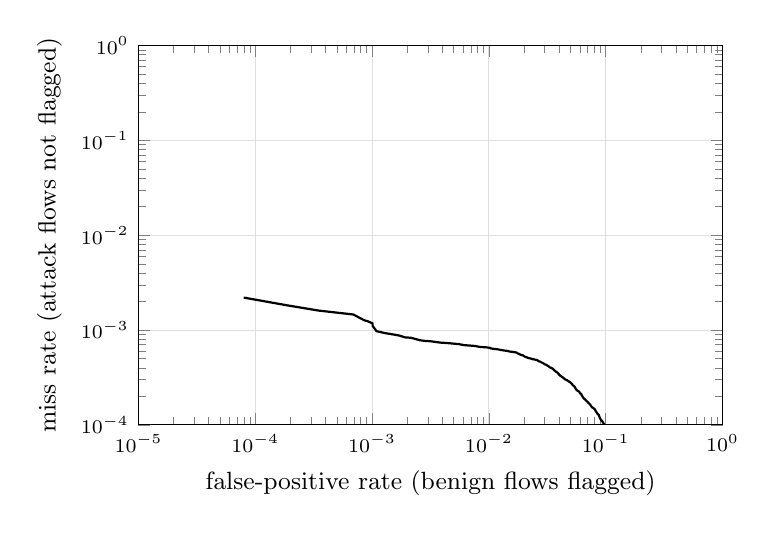
\begin{tikzpicture}
\begin{axis}[width=9cm, height=6.4cm, xmode=log, ymode=log, xlabel={false-positive rate (benign flows flagged)}, ylabel={miss rate (attack flows not flagged)}, xmin=1e-5, xmax=1, ymin=1e-4, ymax=1, grid=major, grid style={gray!25}, tick label style={font=\scriptsize}, label style={font=\small}]
\addplot[black, thick, mark=none] coordinates {(7.97724e-05,0.00220097) (0.000186136,0.00182674) (0.00034568,0.00160792) (0.000691361,0.00146013) (0.000850905,0.00127428) (0.000930678,0.00123115) (0.00101045,0.00117406) (0.00101045,0.00110873) (0.00103704,0.0010618) (0.00109022,0.000974264) (0.00127636,0.000931767) (0.00146249,0.000905761) (0.00170181,0.000877218) (0.00191454,0.000837892) (0.00215385,0.000829647) (0.00233999,0.000806812) (0.00255272,0.000782709) (0.00279203,0.000770658) (0.0031909,0.000761778) (0.00353658,0.000747824) (0.00385567,0.000737675) (0.0043343,0.000730698) (0.00481293,0.000723086) (0.00513202,0.000717378) (0.00553089,0.000711669) (0.00587657,0.000700886) (0.00622225,0.000692641) (0.00680724,0.000687566) (0.00731247,0.000683126) (0.00773792,0.000677418) (0.00813678,0.000667904) (0.00856224,0.000662829) (0.00943973,0.000658389) (0.0101577,0.000650144) (0.0104502,0.000639995) (0.010982,0.000634286) (0.011434,0.000630481) (0.0121254,0.000624772) (0.0125243,0.000618429) (0.0130561,0.000613355) (0.0136943,0.000607646) (0.0143324,0.000603206) (0.0148377,0.000596863) (0.0154227,0.000591155) (0.0160874,0.000588618) (0.0166724,0.000584812) (0.0173638,0.000577201) (0.0177361,0.000566418) (0.0181083,0.000560075) (0.0184008,0.000554366) (0.0189061,0.000546121) (0.0194645,0.000542949) (0.0199165,0.000532801) (0.0204749,0.000522018) (0.0210599,0.000516943) (0.0217779,0.000506795) (0.0227085,0.000502355) (0.0232404,0.000496646) (0.0238254,0.00049284) (0.0248624,0.0004884) (0.0257133,0.00048396) (0.0262185,0.000476349) (0.0268035,0.000469372) (0.0274949,0.000464298) (0.0278672,0.000459858) (0.0283192,0.000455418) (0.028984,0.000449075) (0.029569,0.000442732) (0.0300476,0.000435755) (0.0309783,0.00043068) (0.0314303,0.000424972) (0.0318824,0.000419263) (0.0324674,0.000414823) (0.0330258,0.000406578) (0.0337437,0.000401503) (0.0345149,0.000396429) (0.0351264,0.000391989) (0.035871,0.000383109) (0.0363496,0.000376132) (0.0368283,0.000371058) (0.0375196,0.00036408) (0.0382376,0.000359006) (0.0388492,0.000352663) (0.0394873,0.000345686) (0.0399394,0.000338709) (0.0405776,0.000331732) (0.0415348,0.000325389) (0.0424389,0.00031968) (0.0431569,0.000314606) (0.0440344,0.000308897) (0.0444598,0.000304457) (0.0453639,0.000300652) (0.0465339,0.000296846) (0.0472784,0.000292406) (0.0483952,0.000287332) (0.0492993,0.000282892) (0.0501502,0.000278452) (0.0506289,0.000274646) (0.0514798,0.000269572) (0.0521977,0.000262595) (0.0532082,0.000258155) (0.0540591,0.000253715) (0.0544314,0.000249275) (0.0551759,0.000242297) (0.0557875,0.000237223) (0.0567713,0.000231515) (0.0585263,0.00022644) (0.05959,0.000222) (0.060175,0.000215657) (0.061797,0.000211852) (0.0620895,0.000207412) (0.0627011,0.000202337) (0.0637115,0.000197263) (0.0644295,0.000192189) (0.0655995,0.000188383) (0.0672481,0.000183309) (0.0686574,0.000178234) (0.0701199,0.000174429) (0.0713165,0.000169989) (0.0728588,0.000166183) (0.0742681,0.000161109) (0.0751722,0.000157303) (0.0763688,0.000153497) (0.0784694,0.000150326) (0.080384,0.00014652) (0.081421,0.000143349) (0.0821124,0.000139543) (0.0835483,0.000135737) (0.0851703,0.000130663) (0.087138,0.000127492) (0.088308,0.000121783) (0.0896907,0.000116709) (0.0911001,0.000112903) (0.093573,0.000109097) (0.0954078,0.000104657) (0.097668,9.9583e-05) (0.10038,9.5143e-05) (0.101444,9.00687e-05) (0.10405,8.49944e-05) (0.106177,8.05544e-05) (0.109288,7.67486e-05) (0.111415,7.16744e-05) (0.114473,6.72344e-05) (0.117319,6.34286e-05) (0.119526,5.89886e-05) (0.121839,5.51829e-05) (0.124525,5.01086e-05) (0.127955,4.63029e-05) (0.130002,4.18629e-05) (0.133246,3.74229e-05) (0.137022,3.23486e-05) (0.143511,2.79086e-05) (0.145585,2.34686e-05) (0.150238,1.96629e-05) (0.155795,1.64914e-05) (0.158534,1.20514e-05)};
\end{axis}
\end{tikzpicture}
\caption{Detection-error trade-off curve of the XGBoost detector for attack versus benign on the full test split, scored by one minus the probability of the benign class: miss rate against false-positive rate, both on logarithmic axes. A curve closer to the lower left is better. The area under the corresponding ROC curve is 0.99996 and the average precision 0.999999.}
\label{fig:roc}
\end{figure}


\subsection{Confidence calibration and the confidence gate}
\label{sec:gate}
Confidence is informative here: among alerts, real attacks have median confidence 1.0000 and false alarms 0.7583, and the area under the ROC curve of confidence for separating them is 0.9893. Figure~\ref{fig:reliability} is the reliability diagram of the shipped detector. Nearly all flows (1,559,351 of 1,614,182) fall in the top confidence bin, where mean confidence is 0.9999 and observed accuracy 0.9994. The calibration error is small: ECE is 0.0035 before and 0.0033 after temperature scaling with $T=0.917$ (this temperature was fitted on the validation data of the development model described below, and is applied here unchanged). The diagram also shows where the detector is overconfident: in the bin of 3,387 flows with confidence between 0.73 and 0.80 the observed accuracy is only 0.54. These are the alerts a confidence gate should send to a human.

\begin{figure}[htbp]
\centering
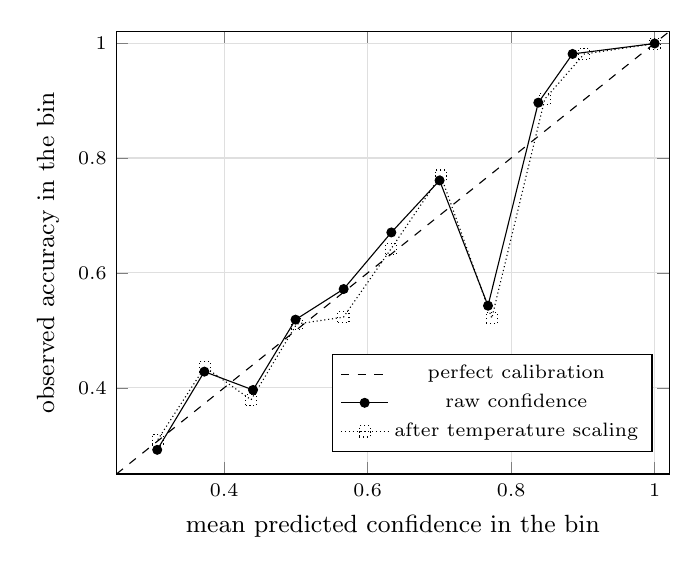
\begin{tikzpicture}
\begin{axis}[
  width=8.6cm, height=7.2cm, xlabel={mean predicted confidence in the bin}, ylabel={observed accuracy in the bin},
  xmin=0.25, xmax=1.02, ymin=0.25, ymax=1.02, grid=both, grid style={gray!25},
  legend style={font=\scriptsize, at={(0.97,0.05)}, anchor=south east},
  tick label style={font=\scriptsize}, label style={font=\small}]
\addplot[black, dashed, mark=none] coordinates {(0.25,0.25) (1.02,1.02)};
\addlegendentry{perfect calibration}
\addplot[black, mark=*, mark size=1.6pt] coordinates {(0.3068,0.2921) (0.3725,0.4282) (0.4403,0.3963) (0.4995,0.5187) (0.5666,0.5720) (0.6330,0.6705) (0.7002,0.7610) (0.7677,0.5430) (0.8378,0.8964) (0.8855,0.9812) (0.9999,0.9994)};
\addlegendentry{raw confidence}
\addplot[black, mark=square, mark size=2pt, densely dotted] coordinates {(0.3077,0.3099) (0.3731,0.4364) (0.4376,0.3792) (0.5011,0.5111) (0.5663,0.5230) (0.6327,0.6421) (0.7019,0.7696) (0.7730,0.5213) (0.8468,0.9026) (0.9015,0.9809) (0.9999,0.9992)};
\addlegendentry{after temperature scaling}
\end{axis}
\end{tikzpicture}
\caption{Reliability diagram of the XGBoost detector on the full test split (15 equal-width bins; bins with fewer than 30 flows are not drawn). Points close to the dashed diagonal are well calibrated.}
\label{fig:reliability}
\end{figure}

To choose a confidence threshold without touching the test split we trained a development model, held out validation data from both training and test, fitted the temperature on validation, and fixed the selection rule beforehand: choose the largest $\tau$ that keeps at least 95\% of real-attack autonomy on validation. Temperature scaling improved validation calibration (ECE 0.0409 to 0.0288; NLL 0.1504 to 0.1495); on test, ECE of the development model was 0.0033 raw and 0.0030 calibrated, while NLL moved slightly the wrong way (0.0204 to 0.0210), so the calibration gain is small and mainly on validation. The rule selected $\tau=0.7$ (Figure~\ref{fig:gate}).

\begin{figure}[htbp]
\centering
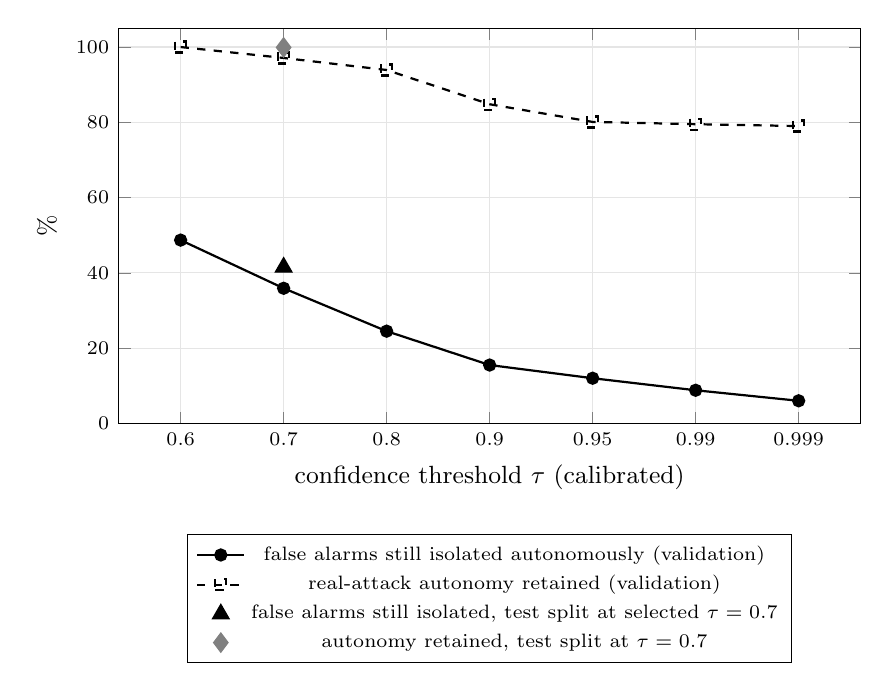
\begin{tikzpicture}
\begin{axis}[
  width=11cm, height=6.6cm, xlabel={confidence threshold $\tau$ (calibrated)}, ylabel={\%},
  xtick={1,2,3,4,5,6,7}, xticklabels={0.6,0.7,0.8,0.9,0.95,0.99,0.999}, ymin=0, ymax=105,
  legend style={font=\scriptsize, at={(0.5,-0.28)}, anchor=north, legend columns=1},
  grid=both, grid style={gray!20}, tick label style={font=\scriptsize}, label style={font=\small}]
\addplot[color=black, mark=*, thick] coordinates {(1,48.7) (2,35.9) (3,24.5) (4,15.5) (5,12.0) (6,8.8) (7,6.0)};
\addlegendentry{false alarms still isolated autonomously (validation)}
\addplot[color=black, mark=square, thick, dashed] coordinates {(1,100.0) (2,97.1) (3,93.9) (4,84.8) (5,80.1) (6,79.5) (7,79.0)};
\addlegendentry{real-attack autonomy retained (validation)}
\addplot[only marks, mark=triangle*, mark size=3.5pt, color=black] coordinates {(2,41.5)};
\addlegendentry{false alarms still isolated, test split at selected $\tau=0.7$}
\addplot[only marks, mark=diamond*, mark size=3.5pt, color=gray] coordinates {(2,99.9)};
\addlegendentry{autonomy retained, test split at $\tau=0.7$}
\end{axis}
\end{tikzpicture}
\caption{Confidence-gate trade-off. $\tau=0.7$ was selected on validation; the triangle and diamond are the single test-split scores at that threshold. Unsafe autonomous actions are 0 at every $\tau$.}
\label{fig:gate}
\end{figure}

Scored once on the untouched test split, the gate left 41.5\% (40.0--43.2\%, range over five context seeds) of the development model's 1,558 false alarms with autonomous isolation, against 50.5\% (48.8--52.1\%) without the gate, while the system still acted autonomously on 99.9\% of the real attacks it would otherwise handle alone. The gate is therefore a modest improvement, not a cure: more than 40\% of false alarms are still isolated without a human. The gate is off by default in the shipped system and is an opt-in setting.

\subsection{Patient-safety behaviour of the decision layer}
\label{sec:safety}
Every one of the 1,614,182 test flows is one trial. The XGBoost detector, Risk Engine and Policy Engine are the real implementations. The dataset has no clinical context, so each trial draws a device context uniformly over three criticality levels crossed with patient-dependent yes or no, and the three language-model-backed agents are replaced by deterministic stand-ins that read the detector's output and the sampled context. The whole experiment is repeated over five context seeds. There are about 262,000 high-stakes trials (a real attack on a HIGH-criticality, patient-dependent device) per seed, and 1,312,874 over the five seeds. Table~\ref{tab:systems} gives the counts behind each rate, and Figure~\ref{fig:systems} draws them.

\begin{table}[htbp]
\centering
\caption{Response systems on the full test split. Counts are for the first context seed; rates are the mean over five seeds (range in brackets).}
\label{tab:systems}
\small
\begin{tabular}{@{}L{3.6cm}C{1.9cm}C{3.6cm}C{3.4cm}@{}}
\toprule
System & Acts without a human? & Unsafe autonomous actions: count / high-stakes trials (rate) & Unnecessary isolations: count / false alarms (rate) \\
\midrule
Detection only & never acts & not applicable & not applicable \\
Fixed response & always & 262,380 / 263,116 (99.72\%; 99.70--99.75) & 1,174 / 1,174 (100.00\%) \\
Detection + Risk Engine & always & 262,380 / 263,116 (99.72\%; 99.70--99.75) & 1,174 / 1,174 (100.00\%) \\
Detection + agentic layer & policy decides & 0 / 263,116 (0.00\%) & 575 / 1,174 (50.48\%; 48.98--52.81) \\
\textbf{Full system} & policy decides & \textbf{0 / 263,116 (0.00\%)} & \textbf{575 / 1,174 (50.48\%; 48.98--52.81)} \\
\bottomrule
\end{tabular}
\end{table}

\begin{figure}[htbp]
\centering
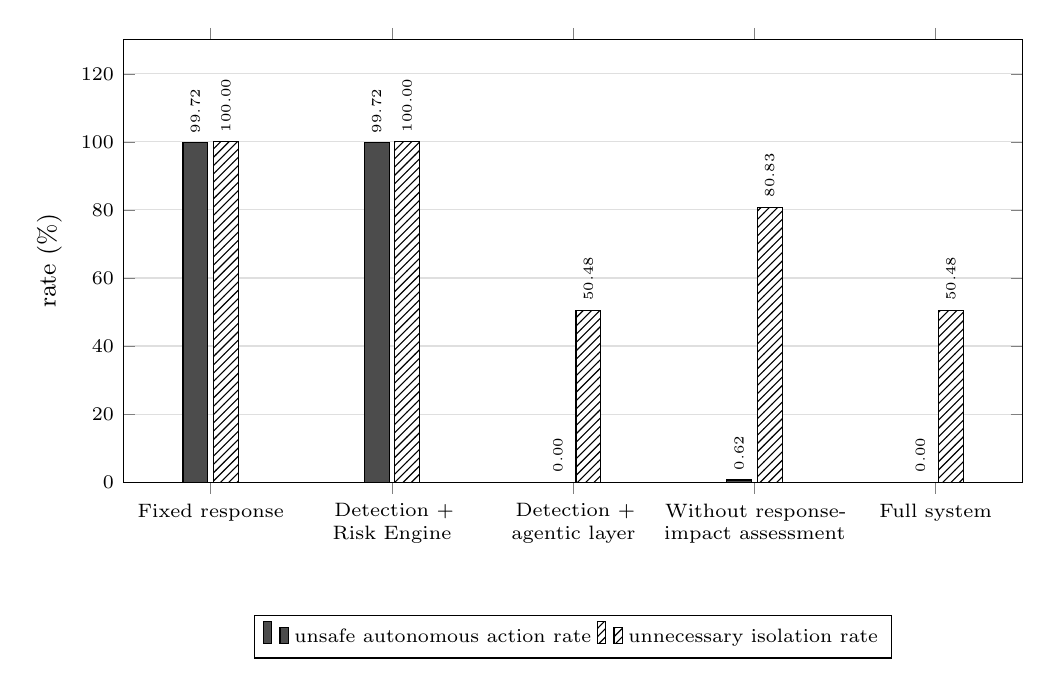
\begin{tikzpicture}
\begin{axis}[
  ybar, width=13cm, height=7.2cm, bar width=9pt, ymin=0, ymax=130, enlarge x limits=0.12,
  symbolic x coords={Fixed response,Detection + Risk Engine,Detection + agentic layer,Without response-impact assessment,Full system},
  xtick=data, xticklabel style={font=\scriptsize, text width=2.3cm, align=center},
  ylabel={rate (\%)}, nodes near coords, nodes near coords style={font=\tiny, rotate=90, anchor=west, /pgf/number format/fixed, /pgf/number format/precision=2, /pgf/number format/fixed zerofill},
  legend style={font=\scriptsize, at={(0.5,-0.3)}, anchor=north, legend columns=2},
  ymajorgrids, grid style={gray!25}, tick label style={font=\scriptsize}, label style={font=\small}]
\addplot[fill=black!70, draw=black] coordinates {(Fixed response,99.72) (Detection + Risk Engine,99.72) (Detection + agentic layer,0) (Without response-impact assessment,0.62) (Full system,0)};
\addlegendentry{unsafe autonomous action rate}
\addplot[fill=white, draw=black, postaction={pattern=north east lines}] coordinates {(Fixed response,100) (Detection + Risk Engine,100) (Detection + agentic layer,50.48) (Without response-impact assessment,80.83) (Full system,50.48)};
\addlegendentry{unnecessary isolation rate}
\end{axis}
\end{tikzpicture}
\caption{Safety of the response systems on the full test split (mean over five context seeds). The numbers above the bars are the rates; a label of 0.00 is a measured zero (0 of 263,116 high-stakes trials in the first seed), so the bar has no height. ``Detection only'' is left out because it never acts, so neither rate is defined for it. The ``Without response-impact assessment'' system is an ablation of the full system (Table~\ref{tab:ablation}).}
\label{fig:systems}
\end{figure}

A zero in this section is a counted result, not a missing result and not a sign that training failed. The detector is trained once (Section~\ref{sec:detector}); this experiment scores its predictions with the decision layer. For the full system the numerator of the unsafe-action rate is the number of high-stakes attacks for which a disruptive action ran without a human, and it is 0 in every seed, 0 of 1,312,874 over the five seeds. The reason is structural, not statistical: the first Policy Engine rule sends every severe action on a patient-dependent device to a human, so no sample of detections can produce an unsafe autonomous action, and Section~\ref{sec:exhaustive} verifies this by enumerating the inputs. For a rate measured as zero events in $n$ trials, the one-sided 95\% upper confidence bound is about $3/n$ (the rule of three), here $2.3\times10^{-6}$. The ``detection only'' system also shows no unsafe action, but trivially, because it never acts; we therefore mark it as not applicable instead of 0.00\%.

A fixed-response playbook, and the same playbook with a Risk Engine score but no routing, execute a disruptive action without a human on 99.72\% of high-stakes real attacks. The agentic layer with the Policy Engine reduces this to zero. The price is the unnecessary isolation rate: on the roughly half of false alarms that land on contexts the policy lets it handle alone, the system still isolates the device (50.48\%). The denominator of that rate is the 1,174 benign flows the detector flagged, a much smaller sample than the unsafe-action denominator; it is the rate the calibrated gate of Section~\ref{sec:gate} lowers.

\begin{table}[htbp]
\centering
\caption{Ablations of the full system on the same trials. ``Differs'' counts trials per seed in which the decision differs from the full system. Counts are for the first context seed.}
\label{tab:ablation}
\small
\begin{tabular}{@{}L{4.2cm}C{3.1cm}C{3.1cm}C{2.4cm}@{}}
\toprule
Ablation & Unsafe autonomous actions: count / trials (mean rate) & Unnecessary isolations: count / false alarms (mean rate) & Differs (per seed) \\
\midrule
Without healthcare context & 0 / 263,116 (0.00\%) & 575 / 1,174 (50.48\%) & 0 \\
Without clinical criticality & 0 / 263,116 (0.00\%) & 575 / 1,174 (50.48\%) & 0 \\
Without response-impact assessment & 1,655 / 263,116 (0.62\%) & 944 / 1,174 (80.83\%) & 5,211--5,334 \\
Without agentic layer & 262,380 / 263,116 (99.72\%) & 1,174 / 1,174 (100.00\%) & 785,951--787,713 \\
Without blockchain & 0 / 263,116 (0.00\%) & 575 / 1,174 (50.48\%) & 0 \\
Without recovery verification & 0 / 263,116 (0.00\%) & 575 / 1,174 (50.48\%) & 0 \\
\bottomrule
\end{tabular}
\end{table}

Table~\ref{tab:ablation} separates what carries the safety result. Removing the response-impact assessment lets 1,655 high-stakes attacks through (0.62\%) and raises unnecessary isolation to 80.83\%, so that component matters. Removing the agentic layer restores the fixed-response behaviour. In this experiment the agentic layer is a deterministic stand-in that supplies clinical context and a planned action, so this ablation shows that the \emph{context-aware planning layer} is essential, not that a language model is necessary. Removing healthcare context, clinical criticality, the blockchain or recovery verification changes nothing here. For the first two this is structural: the Policy Engine routes on response impact and patient dependency, and the patient-dependency rule already forces approval; for the last two, neither component is on this experiment's decision path (the ledger and recovery are evaluated separately in Sections~\ref{sec:agents} and~\ref{sec:chain}). We report these zeros rather than omit them.

Safety is paid for in human time. In the full system 50.0\% of alerts across all devices wait for a person (785,858 contained autonomously, 786,293 waiting), and on high-stakes devices every alert waits (262,215 of 262,215 detected attacks). At the runtime confidence threshold the detector misses 4,424 attack flows overall (708 on high-stakes devices), which no response layer can recover; these shares use three context seeds. The delay model in Section~\ref{sec:compare-cost} uses an \emph{assumed} approval time, since the project has no measurement of one.

\subsection{Sensitivity to the clinical device mix}
\label{sec:sensitivity}
The safety study of Section~\ref{sec:safety} assumes one device mix: criticality uniform, half the devices patient-dependent. A reviewer can fairly ask whether the conclusion depends on that choice, so we repeated the comparison while changing the share of patient-dependent devices from 0 to 100\% (criticality uniform) and the share of HIGH-criticality devices from 0 to 100\% (half the devices patient-dependent). Each setting is scored on a sample of 121,174 trials: all 1,174 detector false alarms plus 120,000 randomly chosen other test flows (the full 1.6 million flows were used in Section~\ref{sec:safety}; a sample keeps eleven settings affordable, and all reported quantities are conditional rates, so including every false alarm does not bias them). Table~\ref{tab:sens} and Figure~\ref{fig:sens} give the results.

\begin{table}[htbp]
\centering
\caption{Sensitivity to the clinical device mix (121,174 sampled trials per row, 1,174 of them false alarms). ``Unsafe'' counts disruptive autonomous actions on high-stakes real attacks; ``isolated'' counts false alarms isolated without a human.}
\label{tab:sens}
\footnotesize
\begin{tabular}{@{}L{1.5cm}C{1.5cm}C{1.5cm}C{1.5cm}C{1.7cm}C{1.9cm}C{1.7cm}@{}}
\toprule
Device mix & High-stakes trials & Unsafe: fixed response & Unsafe: full system & Unsafe: no response impact & False alarms isolated: full system & Autonomy retained: full system \\
\midrule
\multicolumn{7}{@{}l}{\textit{Patient-dependent share (criticality uniform)}}\\
0\% & 0 & not defined & not defined & not defined & 1,174 / 1,174 & 100.0\% \\
10\% & 3,799 & 3,786 & 0 & 22 & 1,075 / 1,174 & 90.0\% \\
25\% & 9,616 & 9,585 & 0 & 66 & 905 / 1,174 & 75.0\% \\
50\% & 19,295 & 19,246 & 0 & 132 & 611 / 1,174 & 50.1\% \\
75\% & 29,164 & 29,088 & 0 & 184 & 283 / 1,174 & 25.0\% \\
90\% & 35,181 & 35,090 & 0 & 222 & 130 / 1,174 & 9.9\% \\
100\% & 39,142 & 39,043 & 0 & 246 & 0 / 1,174 & 0.0\% \\
\multicolumn{7}{@{}l}{\textit{HIGH-criticality share (half of devices patient-dependent)}}\\
0\% & 0 & not defined & not defined & not defined & 601 / 1,174 & 50.0\% \\
33\% & 19,595 & 19,554 & 0 & 115 & 586 / 1,174 & 50.0\% \\
60\% & 35,192 & 35,091 & 0 & 214 & 595 / 1,174 & 50.0\% \\
100\% & 58,621 & 58,451 & 0 & 355 & 582 / 1,174 & 50.1\% \\
\bottomrule
\end{tabular}
\end{table}

\begin{figure}[htbp]
\centering
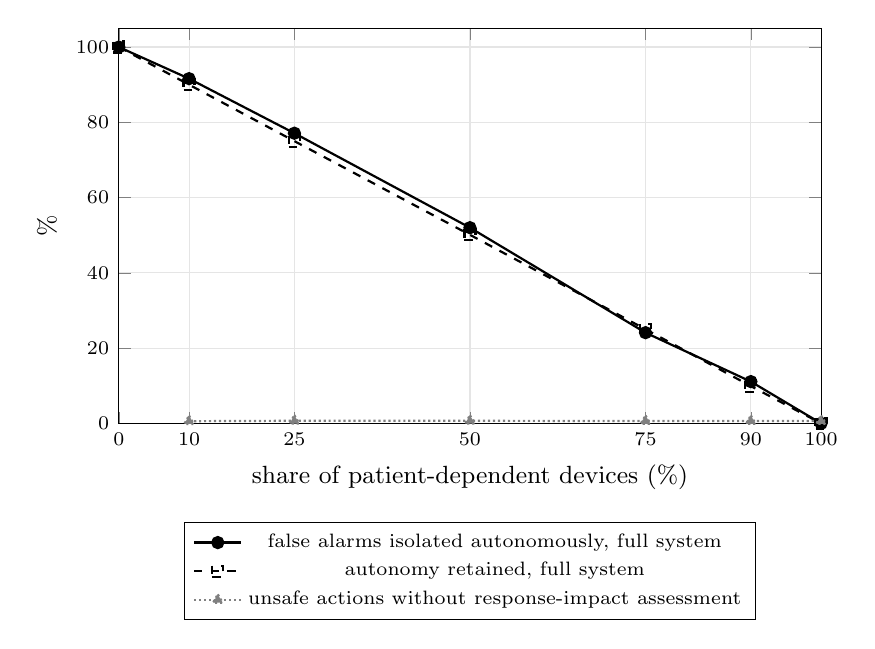
\begin{tikzpicture}
\begin{axis}[
  width=10.5cm, height=6.6cm, xlabel={share of patient-dependent devices (\%)}, ylabel={\%},
  xmin=0, xmax=100, ymin=0, ymax=105, xtick={0,10,25,50,75,90,100},
  legend style={font=\scriptsize, at={(0.5,-0.25)}, anchor=north, legend columns=1},
  grid=both, grid style={gray!20}, tick label style={font=\scriptsize}, label style={font=\small}]
\addplot[black, mark=*, thick] coordinates {(0,100) (10,91.6) (25,77.1) (50,52.0) (75,24.1) (90,11.1) (100,0)};
\addlegendentry{false alarms isolated autonomously, full system}
\addplot[black, mark=square, thick, dashed] coordinates {(0,100) (10,90.0) (25,75.0) (50,50.1) (75,25.0) (90,9.9) (100,0)};
\addlegendentry{autonomy retained, full system}
\addplot[gray, mark=triangle*, thick, densely dotted] coordinates {(10,0.58) (25,0.69) (50,0.68) (75,0.63) (90,0.63) (100,0.63)};
\addlegendentry{unsafe actions without response-impact assessment}
\end{axis}
\end{tikzpicture}
\caption{Effect of the share of patient-dependent devices on the full system. Unsafe autonomous actions of the full system are zero at every share and are therefore not drawn; the dotted line shows the unsafe rate of the ablation without response-impact assessment.}
\label{fig:sens}
\end{figure}

Three things follow from Table~\ref{tab:sens}. First, the safety result does not depend on the mix: the full system has zero unsafe autonomous actions in every setting that contains a high-stakes device, while the fixed-response baseline is unsafe on 99.7--99.8\% of high-stakes attacks in all of them. Second, the response-impact assessment keeps mattering at every mix: without it between 0.6\% and 0.7\% of high-stakes attacks get through, in proportion to the number of such attacks. Third, and this is the honest cost, the autonomy the system retains falls almost linearly with the share of patient-dependent devices, because every action on such a device waits for a person; at 100\% patient-dependent devices the system never acts alone and every false alarm is a task for a human, but also never isolates a device unnecessarily. The 50\% autonomy of the base setting is therefore not a property of the framework but of the assumed mix, and a hospital with mostly patient-dependent devices should expect far more approvals. The HIGH-criticality share has almost no effect on autonomy, because routing depends on patient dependency and not on criticality alone: a HIGH-criticality device without a patient attached is still handled autonomously.

\subsection{Exhaustive verification of the decision rules}
\label{sec:exhaustive}
The experiments above sample trials from a dataset, so at best they show that nothing unsafe happened in $n$ trials. The Risk Engine and Policy Engine are small enough to do better. We enumerated every combination of the eleven response actions, three device criticalities, two patient-dependency values, four stated clinical-impact levels, four threat-severity levels and three threat-confidence values (3,168 inputs), called the real engines on each, and counted the outcomes (Table~\ref{tab:exhaustive}).

\begin{table}[htbp]
\centering
\caption{Policy decisions over all 3,168 inputs, by device context. ``Autonomous'' means the system acts without a human; ``human'' means the action waits for approval.}
\label{tab:exhaustive}
\small
\begin{tabular}{@{}L{4.6cm}C{2.2cm}C{2.2cm}C{2.2cm}@{}}
\toprule
Device context & Inputs & Autonomous & Human \\
\midrule
Low criticality, not patient-dependent & 528 & 528 & 0 \\
Medium criticality, not patient-dependent & 528 & 528 & 0 \\
HIGH criticality, not patient-dependent & 528 & 528 & 0 \\
Low criticality, patient-dependent & 528 & 144 & 384 \\
Medium criticality, patient-dependent & 528 & 144 & 384 \\
HIGH criticality, patient-dependent & 528 & 0 & 528 \\
\midrule
Total & 3,168 & 1,872 & 1,296 \\
\bottomrule
\end{tabular}
\end{table}

Three properties hold over the whole input space. No severe action (shutdown, critical isolation, segment quarantine or failover) is ever autonomous on a patient-dependent device (0 violations among 576 such inputs). No action of any tier is ever autonomous on a HIGH-criticality, patient-dependent device (0 violations among 528 inputs; the only autonomous actions on patient-dependent devices in Table~\ref{tab:exhaustive} are the non-disruptive ones, such as rotating credentials, on low- and medium-criticality devices). And the decision does not depend on the stated threat severity or the confidence: for every fixed action, criticality, dependency and clinical-impact value, all twelve severity-and-confidence combinations gave the same routing. This is a statement about every input, not a sample, which is why the zero unsafe actions of Section~\ref{sec:safety} is a consequence of the rules and not of the data. The table also shows the design choice that a reviewer should know about: HIGH-criticality devices that no patient depends on are handled fully autonomously, including severe actions, because the registry says nothing clinical is at stake.

\subsection{The agentic layer under injected faults}
\label{sec:agents}
To test the claim that no agent can by itself cause harm, the five agents were driven by a scripted, deliberately misbehaving client through the real orchestrator, engines and simulated devices. Ten behaviours were run on three simulated devices: an infusion pump (low criticality, no patient attached), an ECG monitor, and a ventilator (the only HIGH-criticality, patient-dependent device in the simulated hospital). Table~\ref{tab:faults} lists the outcomes; each cell is one deterministic run, so there is no variance to report.

\begin{table}[htbp]
\centering
\caption{Outcome per injected behaviour and device. Auto: resolved or reopened with the system acting alone. Human: held for approval, device untouched. Stall: the incident stopped safely.}
\label{tab:faults}
\small
\begin{tabular}{@{}L{6.2cm}C{1.9cm}C{1.9cm}C{2.4cm}@{}}
\toprule
Injected behaviour & Pump & ECG & Ventilator \\
\midrule
Honest agents (reference) & Auto & Human & Human \\
Context agent claims low criticality, no patient dependency & Auto & Human & Human \\
Same lie, planner also recommends shutdown & Auto (off) & Human & Human \\
Planner recommends shutdown with a false ``low'' impact & Auto (off) & Human & Human \\
Planner understates the clinical impact of isolation & Auto & Human & Human \\
Prompt injection obeyed (text in traffic tells the model to downgrade and shut down) & Auto & Human & Human \\
Every agent returns unparseable text & Stall & Stall & Stall \\
Planner returns an action outside the vocabulary & Stall & Stall & Stall \\
Investigation answers about a different incident & Stall & Stall & Stall \\
Recovery agent claims success while the attack persists & Auto, reopened & Human & Human \\
\bottomrule
\end{tabular}
\end{table}

Across the 30 runs, no unsafe autonomous action took effect on the ventilator and no incident was falsely closed; 9 runs stalled safely and 14 were routed to a human. The infusion pump is acted on autonomously by design: its registry entry allows it, and the lie in the model's output could not make that more or less safe. To see what the guards add, the same 30 runs were repeated with the three guards of Section~\ref{sec:method} switched off (Figure~\ref{fig:guards}); only those three checks differ.

\begin{figure}[htbp]
\centering
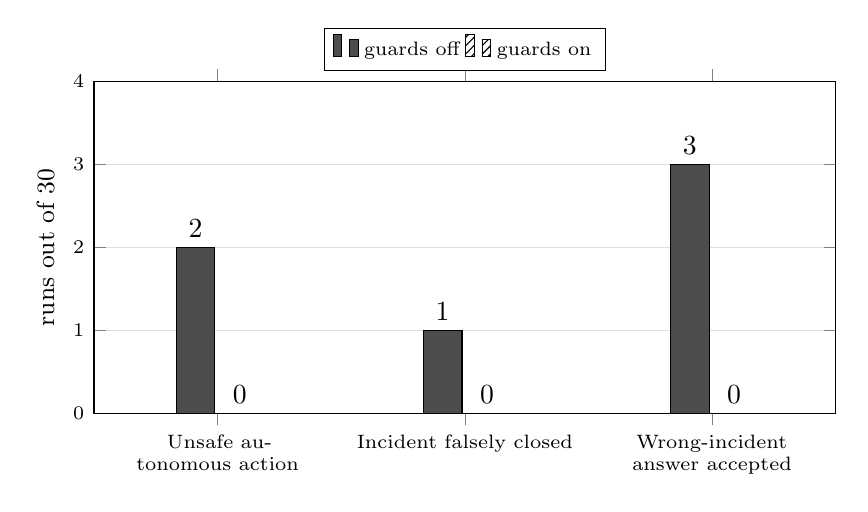
\begin{tikzpicture}
\begin{axis}[
  ybar, width=11cm, height=5.8cm, bar width=14pt, ymin=0, ymax=4, ytick={0,1,2,3,4},
  symbolic x coords={Unsafe autonomous action,Incident falsely closed,Wrong-incident answer accepted},
  xtick=data, xticklabel style={font=\scriptsize, text width=3cm, align=center}, ylabel={runs out of 30},
  nodes near coords, legend style={font=\scriptsize, at={(0.5,1.03)}, anchor=south, legend columns=2},
  ymajorgrids, grid style={gray!25}, tick label style={font=\scriptsize}, label style={font=\small}, enlarge x limits=0.25]
\addplot[fill=black!70, draw=black] coordinates {(Unsafe autonomous action,2) (Incident falsely closed,1) (Wrong-incident answer accepted,3)};
\addlegendentry{guards off}
\addplot[fill=white, draw=black, postaction={pattern=north east lines}] coordinates {(Unsafe autonomous action,0) (Incident falsely closed,0) (Wrong-incident answer accepted,0)};
\addlegendentry{guards on}
\end{axis}
\end{tikzpicture}
\caption{Effect of the grounding guards over the same 30 fault-injected runs. A label of 0 is a measured zero.}
\label{fig:guards}
\end{figure}

With the guards off, two runs took an unsafe autonomous action (the context-lie case, and the context-lie-plus-shutdown case), one incident was falsely closed (the recovery lie), and three answers about the wrong incident were accepted. With the guards on all four counts are zero. These runs show how the architecture behaves under scripted worst cases; they do not show how often a real model misbehaves. A live-model evaluation harness exists, but our attempts to complete it were stopped by the model provider's overload and quota errors, so no live-model figure is reported.

\subsection{Blockchain provenance on a real Fabric network}
\label{sec:chain}
The measurements use real Fabric binaries driven through the backend's own client; nothing is mocked. Table~\ref{tab:integrity} lists the integrity checks, all of which passed. Beyond these checks, all 142 blocks (194 transactions) were fetched from the Hospital peer and re-verified with an independent implementation of Fabric's block hashing. The genuine chain verified. Editing one byte of one transaction in block 70 (on a copy) was detected at block 70 by the data hash. When the attacker also recomputed that block's own data hash, the edit was still detected, at block 71, because the next block's previous-hash no longer matched. All 188 transactions that the client reported as committed were found as valid on the ledger; the 2 invalid transactions on the chain (an endorsement-policy failure and a read conflict) were produced on purpose by the checks, stay on the chain flagged, and never changed state.

\begin{table}[htbp]
\centering
\caption{Ledger integrity checks (all passed).}
\label{tab:integrity}
\small
\begin{tabular}{@{}C{0.8cm}L{11.8cm}@{}}
\toprule
\# & Check \\
\midrule
1 & A duplicate incident id is rejected (the incident record is write-once). \\
2 & A decision for an unknown incident is rejected. \\
3 & An invalid response-action category is rejected. \\
4 & The evidence-verification function accepts the recorded evidence hash. \\
5 & The evidence-verification function rejects evidence altered by one field. \\
6 & The Hospital and SecurityOps peers return the same answer. \\
7 & Two simultaneous writers of one incident id: exactly one is committed, and only that record is on the ledger. \\
8 & A transaction endorsed by one organisation only is invalidated by the majority policy and writes no state. \\
\bottomrule
\end{tabular}
\end{table}

\begin{table}[htbp]
\centering
\caption{Ledger latency (ms, sequential). A write returns only after both peers have committed. $n$ is the number of operations timed.}
\label{tab:chainlat}
\small
\begin{tabular}{@{}L{7.2cm}cccc@{}}
\toprule
Operation & $n$ & p50 & p95 & max \\
\midrule
Fabric command-line spawn alone (floor) & 20 & 65 & 188 & 239 \\
Write of an incident record & 40 & 1114 & 1139 & 1147 \\
Query sees a committed write & 20 & 87 & 112 & 127 \\
Read: evidence verification & 40 & 89 & 108 & 115 \\
Full five-record incident lifecycle & 10 & 5578 & 5610 & 5617 \\
\bottomrule
\end{tabular}
\end{table}

Table~\ref{tab:chainlat} shows that a write takes about 1.1~s at the median, mostly the 1~s orderer batch timeout plus the wait for both peers; a full lifecycle takes about 5.6~s. Because provenance is written through the outbox off the response path, these latencies do not delay containment. Figure~\ref{fig:conc} shows committed throughput with concurrent clients: 0.90, 1.78, 3.36 and 5.99 transactions per second for 1, 2, 4 and 8 clients, with no failed transaction among 24 submitted at each level and median latency rising from 1111 to 1321~ms. Scaling is near linear to four clients and then sub-linear, as expected on a 2-CPU host where every call spawns a command-line process.

\begin{figure}[htbp]
\centering
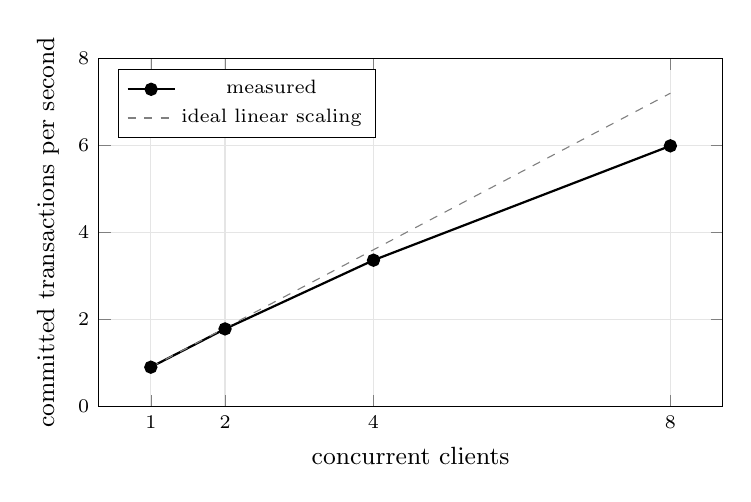
\begin{tikzpicture}
\begin{axis}[
  width=9.5cm, height=6cm, xlabel={concurrent clients}, ylabel={committed transactions per second},
  xtick={1,2,4,8}, ymin=0, ymax=8, grid=both, grid style={gray!20},
  legend style={font=\scriptsize, at={(0.03,0.97)}, anchor=north west},
  tick label style={font=\scriptsize}, label style={font=\small}]
\addplot[color=black, mark=*, thick] coordinates {(1,0.90) (2,1.78) (4,3.36) (8,5.99)};
\addlegendentry{measured}
\addplot[color=gray, dashed, mark=none] coordinates {(1,0.90) (2,1.80) (4,3.60) (8,7.20)};
\addlegendentry{ideal linear scaling}
\end{axis}
\end{tikzpicture}
\caption{Committed throughput of the real Fabric network versus concurrent clients (24 transactions per level, none failed).}
\label{fig:conc}
\end{figure}

The first run of this evaluation also exposed a defect. The client reported success once a transaction was endorsed and handed to the orderer, not once it was committed. A transaction invalidated at commit would still have been reported as committed, so the outbox could mark a record confirmed that never reached the ledger. The invoke script now waits for both peers' commit events and exits non-zero for an invalidated transaction; the latencies above are measured with the fix, and the checks and integration tests guard against a regression.

\subsection{Pipeline latency}
\label{sec:latency}
Table~\ref{tab:pipe} gives the in-process compute cost of the deterministic part of the pipeline. The decision path (Risk plus Policy) costs about 0.016~ms at the median, and the detector scores a flow in 0.77~ms (batch throughput 32,311 flows per second), so neither is a bottleneck; the language-model calls would dominate in a live deployment and are not included.

\begin{table}[htbp]
\centering
\caption{In-process latency of the deterministic pipeline stages (ms); $n$ is the number of timed calls.}
\label{tab:pipe}
\small
\begin{tabular}{@{}L{6.6cm}cccc@{}}
\toprule
Stage & p50 & p95 & p99 & $n$ \\
\midrule
Risk Engine + Policy Engine, per incident & 0.016 & 0.025 & 0.053 & 3,000 \\
Detector, one flow & 0.765 & 0.969 & 1.393 & 300 \\
\bottomrule
\end{tabular}
\end{table}

\subsection{Analysis and limitations}
\label{sec:limits}
The results support four claims. On real data, the decision layer never lets a disruptive autonomous action reach a registry-flagged high-stakes device, whether the clinical context is supplied by a stand-in (Section~\ref{sec:safety}), by a different device mix (Section~\ref{sec:sensitivity}), or by a scripted lying agent (Section~\ref{sec:agents}); this holds for every input of the rule tables (Section~\ref{sec:exhaustive}). The detector's performance is stable across training seeds and classifiers (Section~\ref{sec:robust}). The ledger detects tampering of the kind we tried. And the guards close exactly the gaps that a scripted model opens when they are removed.

The results do not support several claims, and a reader should not draw them. The clinical context in the safety studies is sampled, not observed, and the agents in the safety and fault-injection studies are scripted: the results concern the gating logic, not clinical outcomes and not the error rate of a real model. In the fault-injection study only one simulated device is both HIGH-criticality and patient-dependent, so the study alone rests on ten ventilator runs; the exhaustive check of Section~\ref{sec:exhaustive} covers the rule tables but not the integration. The unnecessary-isolation rate of 41.5--50.5\% is a real weakness: a false alarm on a permitted device still causes autonomous isolation, and the cost of safety in human approvals grows with the share of patient-dependent devices (Section~\ref{sec:sensitivity}). The Fabric network has one orderer on one 2-CPU host, with one run and no confidence intervals, so it says nothing about orderer fault tolerance or malicious orderers, and its latencies belong to this deployment rather than to Fabric. The test flows within one capture are strongly correlated, so the bootstrap intervals of Section~\ref{sec:robust} understate the uncertainty across captures. Finally, the system is a research prototype, not a certified medical product.

%% ==========================================================================
\section{Comparisons}
\label{sec:comparison}

We compare the proposed framework with existing work on three axes: detection quality against published detectors (Section~\ref{sec:compare-det}), capabilities against related systems (Section~\ref{sec:compare-cap}), and safety and responsiveness against response baselines and unguarded agents (Section~\ref{sec:compare-cost}). Throughout, figures for other works are \emph{as reported by their authors} and are cited in the table row or cell that uses them; we did not retrain or re-run any other work.

\subsection{Detection quality against published detectors}
\label{sec:compare-det}
Table~\ref{tab:cmpdet} places our XGBoost detector beside L2D2~\cite{akar2025}, the reinforcement-learning hybrid HCLR-IDS~\cite{shaikh2025} and the interpretable XGBoost fusion of Hafid et al.~\cite{hafid2025}, all on CICIoMT2024, and beside two ensemble detectors that use a different dataset (WUSTL-EHMS-2020)~\cite{alsolami2024,abdelhaq2026}, which are listed for context only because their accuracy cannot be compared with ours. Hafid et al.\ use the CIC IoMT 2024 release with a reduced feature set. The last two rows give our result for the main model of Section~\ref{sec:detector} and its mean over five training seeds (Section~\ref{sec:robust}).

\begin{table}[htbp]
\centering
\caption{Detection comparison. Values for other works are quoted from the cited papers; ``this work'' rows are measured on the full official CICIoMT2024 test split.}
\label{tab:cmpdet}
\footnotesize
\begin{tabular}{@{}L{2.1cm}L{2.1cm}L{2.3cm}C{0.9cm}C{1.9cm}L{2.8cm}@{}}
\toprule
Work & Dataset & Model & Classes & Accuracy & Other reported metrics \\
\midrule
L2D2~\cite{akar2025} & CICIoMT2024 & Enhanced LSTM & 19 & 98\% & none extracted \\
HCLR-IDS~\cite{shaikh2025} & CICIoMT2024 & CNN-LSTM, DQN, PPO & 18 & 0.7773 (multi-class); 0.9958 (binary) & Mutual-information feature selection \\
Hafid et al.~\cite{hafid2025} & CIC IoMT 2024 & XGBoost + logistic-regression fusion, SHAP & as in dataset & 0.97 (XGBoost) & Fusion: precision 0.98, recall 0.91; false negatives 361 to 213 \\
Alsolami et al.~\cite{alsolami2024} & WUSTL-EHMS-2020 & Stacked random forest and SVM & binary & 98.88\% & --- \\
Abdelhaq et al.~\cite{abdelhaq2026} & WUSTL-EHMS-2020 & Soft-voting XGBoost and two SVMs & binary & 98.04\% & Validated on TON-IoT and CICIDS 2017 \\
\textbf{This work} (main model) & CICIoMT2024 & XGBoost, 45 features & 19 & \textbf{0.9952} (19-class); 0.9985 (binary) & Macro-F1 0.9263; attack detection 0.9997; benign FPR 0.0509 \\
\textbf{This work} (5 seeds) & CICIoMT2024 & XGBoost, 30,000 rows per class & 19 & 0.9953 $\pm$ 0.0002 & Macro-F1 0.9103 $\pm$ 0.0017 \\
\bottomrule
\end{tabular}
\end{table}

\begin{figure}[htbp]
\centering
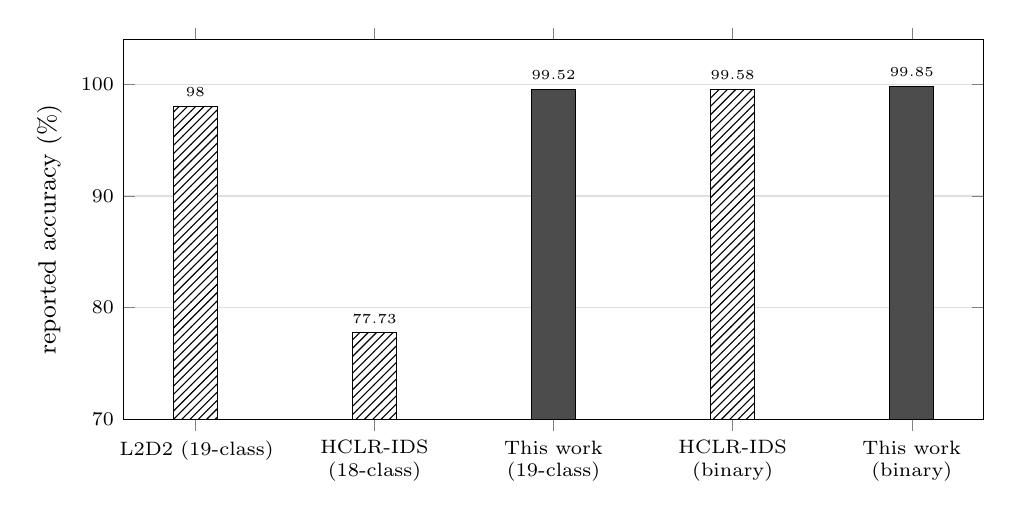
\begin{tikzpicture}
\begin{axis}[
  ybar, width=12.5cm, height=6.4cm, bar width=16pt, ymin=70, ymax=104,
  symbolic x coords={L2D2 (19-class),HCLR-IDS (18-class),This work (19-class),HCLR-IDS (binary),This work (binary)},
  xtick={L2D2 (19-class),HCLR-IDS (18-class),This work (19-class),HCLR-IDS (binary),This work (binary)}, xticklabel style={font=\scriptsize, text width=2.1cm, align=center},
  ylabel={reported accuracy (\%)}, nodes near coords, nodes near coords style={font=\tiny},
  ymajorgrids, grid style={gray!25}, tick label style={font=\scriptsize}, label style={font=\small}]
\addplot[fill=white, draw=black, postaction={pattern=north east lines}, bar shift=0pt] coordinates {(L2D2 (19-class),98.0) (HCLR-IDS (18-class),77.73) (HCLR-IDS (binary),99.58)};
\addplot[fill=black!70, draw=black, bar shift=0pt] coordinates {(This work (19-class),99.52) (This work (binary),99.85)};
\end{axis}
\end{tikzpicture}
\caption{Reported accuracy on CICIoMT2024, multi-class (left three bars) and binary (right two). Hatched bars are quoted from L2D2~\cite{akar2025} and HCLR-IDS~\cite{shaikh2025}; solid bars are measured in this work. The vertical axis starts at 70\%.}
\label{fig:cmpdet}
\end{figure}

On the quoted numbers our detector is on par with or above the others on accuracy (Figure~\ref{fig:cmpdet}), and its 19-class accuracy of 99.52\% compares with 98\% for L2D2 and 77.73\% for the 18-class HCLR-IDS. We do not claim a win. The comparison is indicative only for three reasons: the protocols differ (the other authors' splits, class definitions and preprocessing may not match the official capture-level split we use, and HCLR-IDS counts 18 classes where we count 19); accuracy on this dataset is dominated by the volumetric DDoS and DoS classes; and the figures we could extract from the other papers are accuracies, so they cannot be compared on macro-F1, where our weak classes (ARP spoofing 0.53, vulnerability scanning 0.69) are visible. The contribution of this work is therefore not a new detector but what is built after it.

\subsection{Capability comparison}
\label{sec:compare-cap}
Table~\ref{tab:cap} compares what each system covers. This is where the proposed framework differs from the detection papers~\cite{akar2025,shaikh2025,hafid2025}, from the Fabric prototype for IoMT~\cite{pelekoudas2023}, from the forensic blockchain~\cite{xiao2024}, and from the language-model response agents~\cite{lin2025,gao2026}.

\begin{table}[htbp]
\centering
\caption{Capabilities as described in each cited work's title and abstract. \checkmark{} = addressed; -- = not part of the stated scope (not a defect of that work); $\circ$ = partly, or in simulation only, or not verified from what we read.}
\label{tab:cap}
\footnotesize
\begin{tabular}{@{}L{3.0cm}C{1.15cm}C{1.15cm}C{1.15cm}C{1.15cm}C{1.15cm}C{1.15cm}C{1.15cm}@{}}
\toprule
 & {\scriptsize Real IoMT data} & {\scriptsize Auto- mated response} & {\scriptsize Patient- aware gate} & {\scriptsize LLM agents} & {\scriptsize Output guard} & {\scriptsize Block- chain} & {\scriptsize Ledger tested} \\
\midrule
L2D2~\cite{akar2025} & \checkmark & -- & -- & -- & -- & -- & -- \\
HCLR-IDS~\cite{shaikh2025} & \checkmark & -- & -- & -- & -- & -- & -- \\
Hafid et al.~\cite{hafid2025} & \checkmark & -- & -- & -- & -- & -- & -- \\
Pelekoudas-Oikonomou et al.~\cite{pelekoudas2023} & -- & -- & -- & -- & -- & \checkmark & $\circ$ \\
Xiao et al.~\cite{xiao2024} & -- & -- & -- & -- & -- & \checkmark & $\circ$ \\
IRCopilot~\cite{lin2025} & -- & \checkmark & -- & \checkmark & -- & -- & -- \\
Gao et al.~\cite{gao2026} & -- & \checkmark & -- & \checkmark & -- & -- & -- \\
\textbf{This work} & \checkmark & \checkmark & \checkmark & \checkmark & \checkmark & \checkmark & \checkmark \\
\bottomrule
\end{tabular}
\end{table}

No cited system combines all seven columns, but Table~\ref{tab:cap} is a statement about coverage, not performance: a more specialised work may do its one column better than we do. For example, IRCopilot is evaluated on a response benchmark that we do not use, and Gao et al.\ report recovery-time gains that our framework, which spends human time on purpose, does not aim for.

\subsection{Safety and responsiveness against response baselines}
\label{sec:compare-cost}
No cited work reports an unsafe-autonomous-action rate, so there is no published number to quote for it. The baselines in Table~\ref{tab:cmpsafe} are therefore reference systems implemented in this work to stand for existing practice: a fixed playbook that isolates any attacked device, and a fully manual process (detection only). They are not re-implementations of a particular published system. The figures are those of Section~\ref{sec:safety}.

\begin{table}[htbp]
\centering
\caption{Safety against reference baselines on the full test split (first context seed). The baselines are implemented in this work and are not published systems.}
\label{tab:cmpsafe}
\small
\begin{tabular}{@{}L{3.5cm}C{3.4cm}C{2.4cm}L{3.2cm}@{}}
\toprule
System & Unsafe autonomous actions (of high-stakes attacks) & Alerts waiting for a person & Remaining weakness \\
\midrule
Fixed playbook & 262,380 of 263,116 (99.72\%) & 0\% & Disrupts patient-dependent devices \\
Fully manual (detection only) & 0 of 263,116 (never acts) & 100\% & Every alert waits for a person \\
\textbf{Full system} & \textbf{0 of 263,116 (0.00\%)} & 50.0\% & 41.5--50.5\% of false alarms are isolated \\
\bottomrule
\end{tabular}
\end{table}

A second comparison concerns agents that have no deterministic output guard. IRCopilot~\cite{lin2025} and the fine-tuned agent of Gao et al.~\cite{gao2026} describe no such guard in their abstracts, and we did not run either. As a stand-in for that design we use our own agentic layer with the three guards switched off, run over the same 30 fault-injected cases as Section~\ref{sec:agents}. Table~\ref{tab:cmpguard} is a comparison of guarded and unguarded versions of one system on scripted faults; it says nothing about the quality of the cited agents.

\begin{table}[htbp]
\centering
\caption{Guarded versus unguarded agents over the same 30 fault-injected runs (Section~\ref{sec:agents}). The unguarded configuration stands for agent designs without an output guard such as~\cite{lin2025,gao2026}; it is not a re-implementation of them.}
\label{tab:cmpguard}
\small
\begin{tabular}{@{}L{3.9cm}C{2.5cm}C{2.5cm}C{3.0cm}@{}}
\toprule
Configuration & Unsafe autonomous actions on the ventilator & Incidents falsely closed & Wrong-incident answers accepted \\
\midrule
Unguarded agents (guards off) & 2 of 30 runs & 1 & 3 \\
\textbf{Guarded agents (guards on)} & \textbf{0 of 30 runs} & \textbf{0} & \textbf{0} \\
\bottomrule
\end{tabular}
\end{table}

Safety has a responsiveness cost. The fully manual process is as safe as the full system but makes every alert wait; the fixed playbook never waits but is unsafe (Table~\ref{tab:cmpsafe}). Figure~\ref{fig:wait} shows the mean time before containment under a \emph{modelled} human approval time $D$: pipeline time is measured, the share of alerts that wait is measured (50.0\% overall for the full system, 100\% on high-stakes devices), and $D$ is an assumption because the project has no measurement of a real approval time. Averaged over all devices the full system halves the manual wait; on high-stakes devices it equals the manual wait, by design.

\begin{figure}[htbp]
\centering
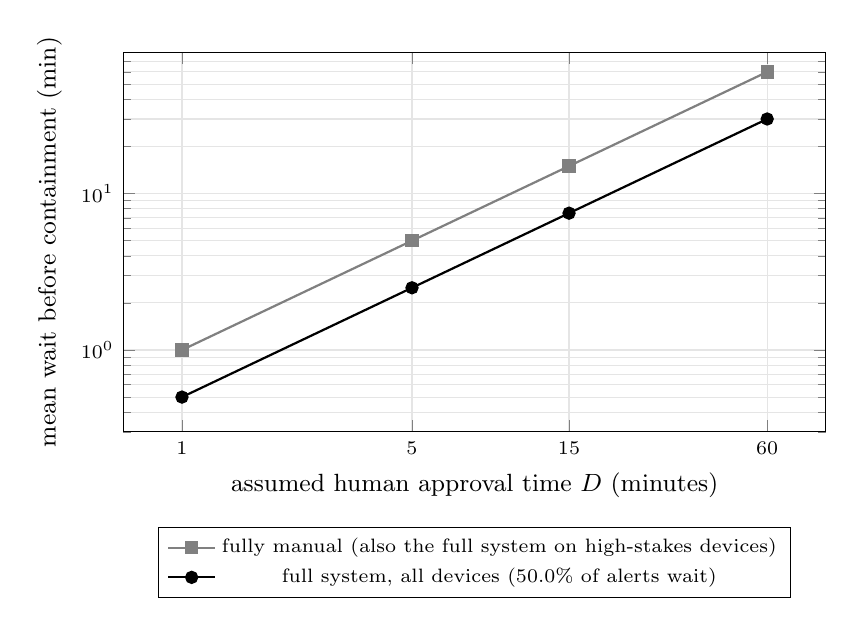
\begin{tikzpicture}
\begin{axis}[
  width=10.5cm, height=6.4cm, xlabel={assumed human approval time $D$ (minutes)}, ylabel={mean wait before containment (min)},
  xmode=log, ymode=log, xtick={1,5,15,60}, xticklabels={1,5,15,60}, ymin=0.3, ymax=80,
  legend style={font=\scriptsize, at={(0.5,-0.25)}, anchor=north},
  grid=both, grid style={gray!20}, tick label style={font=\scriptsize}, label style={font=\small}]
\addplot[color=gray, mark=square*, thick] coordinates {(1,1) (5,5) (15,15) (60,60)};
\addlegendentry{fully manual (also the full system on high-stakes devices)}
\addplot[color=black, mark=*, thick] coordinates {(1,0.5) (5,2.5) (15,7.5) (60,30.0)};
\addlegendentry{full system, all devices (50.0\% of alerts wait)}
\end{axis}
\end{tikzpicture}
\caption{Modelled mean wait before containment against an assumed approval time (fixed playbook: 0, not drawn on the logarithmic axis). The shares of alerts that wait are measured; $D$ is assumed.}
\label{fig:wait}
\end{figure}

\subsection{Discussion}
\label{sec:compare-disc}
Three points follow from the comparisons. First, detection accuracy is no longer the differentiator on CICIoMT2024: the published detectors and ours are all high, and our remaining weaknesses (ARP spoofing, scans) show up only in per-class metrics. Second, the safety result comes from the structure of the system, not from model quality: the Policy Engine's registry-based rule produces the zero unsafe actions regardless of what the agents say (Section~\ref{sec:exhaustive}), and the guards stop wrong agent output from reaching the Policy Engine's inputs. Third, the cost is real and visible: half of alerts wait for a person in the base setting and more in hospitals with many patient-dependent devices (Section~\ref{sec:sensitivity}), and false alarms are still isolated at a rate that the calibrated gate only partly reduces. These are the trade-offs a hospital would have to accept or tune, and they are the questions a deployment study with real clinicians must answer.

%% ==========================================================================
\section{Conclusion}
\label{sec:conclusion}
This paper presented a patient-aware framework that turns detection of attacks on medical devices into a safe and auditable response. Its novelty is the evaluated combination of a real detector, untrusted language-model agents corrected by deterministic guards, rule-based engines that place a human before severe actions on patient-dependent devices, and tamper-evident provenance on a real Fabric network. On the full CICIoMT2024 test split the detector reached 99.52\% accuracy, and across about 1.3 million high-stakes trials the system took no unsafe autonomous action, against 99.72\% for a fixed playbook; an exhaustive check of 3,168 policy inputs confirmed the rule. Under injected faults the guards removed every unsafe action, and every tested ledger tampering was detected. Limits remain: device context and agents were simulated, about half of false alarms are still isolated, and the ledger used one orderer. Future work will evaluate real language models with clinician approval studies on hospital device inventories, and will run the ledger on a multi-orderer network.

%% ==========================================================================
\begin{thebibliography}{99}
\small
\bibitem{naghib2025} A.~Naghib, F.~S. Gharehchopogh, A.~Zamanifar, A comprehensive and systematic literature review on intrusion detection systems in the internet of medical things: current status, challenges, and opportunities, Artificial Intelligence Review 58 (2025) 114. \href{https://doi.org/10.1007/s10462-024-11101-w}{doi:10.1007/s10462-024-11101-w}.

\bibitem{dadkhah2024} S.~Dadkhah, E.~C.~P. Neto, R.~Ferreira, R.~C. Molokwu, S.~Sadeghi, A.~A. Ghorbani, CICIoMT2024: Attack vectors in healthcare devices -- a multi-protocol dataset for assessing IoMT device security, Internet of Things 28 (2024). (Elsevier PII S2542660524002920.) % TODO: add article number / DOI from the publisher page.

\bibitem{akar2025} G.~Akar, S.~Sahmoud, M.~Onat, U.~Cavusoglu, E.~Malondo, L2D2: A novel LSTM model for multi-class intrusion detection systems in the era of IoMT, IEEE Access 13 (2025) 7002--7013. \href{https://doi.org/10.1109/ACCESS.2025.3526883}{doi:10.1109/ACCESS.2025.3526883}.

\bibitem{shaikh2025} J.~A. Shaikh, C.~Wang, M.~W.~U. Sima, M.~Arshad, M.~Owais, D.~S.~M. Hassan, R.~Alkanhel, M.~S.~A. Muthanna, A deep reinforcement learning-based robust intrusion detection system for securing IoMT healthcare networks, Frontiers in Medicine 12 (2025) 1524286. \href{https://doi.org/10.3389/fmed.2025.1524286}{doi:10.3389/fmed.2025.1524286}.

\bibitem{hafid2025} A.~Hafid, M.~Rahouti, M.~Aledhari, Optimizing intrusion detection in IoMT networks through interpretable and cost-aware machine learning, Mathematics 13~(10) (2025) 1574. \href{https://doi.org/10.3390/math13101574}{doi:10.3390/math13101574}.

\bibitem{lin2025} X.~Lin, J.~Zhang, G.~Deng, T.~Liu, T.~Zhang, Q.~Guo, R.~Chen, IRCopilot: Automated incident response with large language models, arXiv:2505.20945 (2025), preprint.

\bibitem{gao2026} Y.~Gao, K.~Hammar, T.~Li, In-context autonomous network incident response: An end-to-end large language model agent approach, arXiv:2602.13156 (2026), preprint.

\bibitem{hasnain2023} M.~Hasnain, F.~R. Albogamy, S.~S. Alamri, I.~Ghani, B.~Mehboob, The Hyperledger Fabric as a blockchain framework preserves the security of electronic health records, Frontiers in Public Health 11 (2023) 1272787. \href{https://doi.org/10.3389/fpubh.2023.1272787}{doi:10.3389/fpubh.2023.1272787}.

\bibitem{pelekoudas2023} F.~Pelekoudas-Oikonomou, J.~C. Ribeiro, G.~Mantas, G.~Sakellari, J.~Gonzalez, Prototyping a Hyperledger Fabric-based security architecture for IoMT-based health monitoring systems, Future Internet 15~(9) (2023) 308. \href{https://doi.org/10.3390/fi15090308}{doi:10.3390/fi15090308}.

\bibitem{vidhya2023} S.~Vidhya, V.~Kalaivani, A blockchain based secure and privacy aware medical data sharing using smart contract and encryption scheme, Peer-to-Peer Networking and Applications (2023). \href{https://doi.org/10.1007/s12083-023-01449-1}{doi:10.1007/s12083-023-01449-1}. % TODO: add volume/pages

\bibitem{mukhopadhyay2021} A.~Mukhopadhyay, R.~Vinayaka, A smart-contract-based blockchain for a healthcare IoT network, International Journal of Electronic Healthcare (2021). \href{https://doi.org/10.1504/IJEH.2021.117122}{doi:10.1504/IJEH.2021.117122}. % TODO: add volume/pages

\bibitem{pranav2026} M.~M. Pranav, S.~Rithan, R.~D.~A. Raj, A.~Pallakonda, R.~M.~R. Yanamala, K.~Prakasha~K., Smart grid cybersecurity against power system MiTM threats and machine learning-based attack classification, Energy Reports (2026). \href{https://doi.org/10.1016/j.egyr.2025.12.035}{doi:10.1016/j.egyr.2025.12.035}. % TODO: add volume/article number

\bibitem{vignes2025} V.~M. Vignes, M.~P. Sri~Harini, R.~Satheesh, V.~Das, S.~Padmanaban, AI-driven cybersecurity framework for anomaly detection in power systems, Scientific Reports (2025). \href{https://doi.org/10.1038/s41598-025-19634-y}{doi:10.1038/s41598-025-19634-y}. % TODO: add volume/article number

\bibitem{alsolami2024} T.~Alsolami, B.~Alsharif, M.~Ilyas, Enhancing cybersecurity in healthcare: Evaluating ensemble learning models for intrusion detection in the Internet of Medical Things, Sensors 24~(18) (2024) 5937. \href{https://doi.org/10.3390/s24185937}{doi:10.3390/s24185937}.

\bibitem{abdelhaq2026} M.~Abdelhaq, S.~Palanisamy, M.~Gopinath, V.~G.~S. Manasa, M.~A. Ram, S.~Khan, et~al., A hybrid XGBoost--SVM ensemble framework for robust cyber-attack detection in the internet of medical things (IoMT), Scientific Reports 16 (2026) 6855. \href{https://doi.org/10.1038/s41598-026-37832-0}{doi:10.1038/s41598-026-37832-0}. % VERIFY the full author list

\bibitem{xiao2024} N.~Xiao, Z.~Wang, X.~Sun, J.~Miao, A novel blockchain-based digital forensics framework for preserving evidence and enabling investigation in industrial Internet of Things, Alexandria Engineering Journal 86 (2024) 631--643. % TODO: add DOI

\end{thebibliography}

\end{document}
